%--------------------------------------------------------------------%
%
% Berkas utama templat LaTeX.
%
% author Petra Barus, Peb Ruswono Aryan
%
%--------------------------------------------------------------------%
%
% Berkas ini berisi struktur utama dokumen LaTeX yang akan dibuat.
%
%--------------------------------------------------------------------%

\documentclass[12pt, a4paper, onecolumn, oneside, final]{report}

%-------------------------------------------------------------------%
%
% Konfigurasi dokumen LaTeX untuk laporan tesis IF ITB
%
% @author Petra Novandi
%
%-------------------------------------------------------------------%
%
% Berkas asli berasal dari Steven Lolong
%
%-------------------------------------------------------------------%

% Ukuran kertas
\special{papersize=210mm,297mm}

% Setting margin
\usepackage[top=3cm,bottom=2.5cm,left=4cm,right=2.5cm]{geometry}

\usepackage{mathptmx}

% Judul bahasa Indonesia
\usepackage[bahasa]{babel}

% Format citation
\usepackage[backend=bibtex,style=alphabetic,citestyle=authoryear]{biblatex}

\usepackage[utf8]{inputenc}
\usepackage{graphicx}
\usepackage{titling}
\usepackage{blindtext}
\usepackage{sectsty}
\usepackage{chngcntr}
\usepackage{etoolbox}
\usepackage{hyperref}       % Package untuk link di daftar isi.
\usepackage{titlesec}       % Package Format judul
\usepackage{parskip}

% Mengatasi bug pada update terbaru titlesec yang menyebabkan section number hilang
\usepackage{etoolbox}

\makeatletter
\patchcmd{\ttlh@hang}{\parindent\z@}{\parindent\z@\leavevmode}{}{}
\patchcmd{\ttlh@hang}{\noindent}{}{}{}
\makeatother

% Line satu setengah spasi
\renewcommand{\baselinestretch}{1.5}

% Setting judul
\chapterfont{\centering \Large}
\titleformat{\chapter}[display]
  {\Large\centering\bfseries}
  {\chaptertitlename\ \thechapter}{0pt}
    {\Large\bfseries\uppercase}

% Setting nomor pada subbsubsubbab
\setcounter{secnumdepth}{3}

\makeatletter

\makeatother

% Counter untuk figure dan table.
\counterwithin{figure}{section}
\counterwithin{table}{section}

\input{config/hypenation-id}

\makeatletter

\makeatother
\makeglossaries

\bibliography{references}
\loadglsentries{glossaries}

\begin{document}
\sloppy

    %Basic configuration
    \title{Sistem Permainan Musik Ekspresif untuk Alat Musik Gesek}
    \date{}
    \author{
        Muhammad Nizami \\
        NIM 23517044
    }

    \pagenumbering{roman}
    \setcounter{page}{0}

    \clearpage
\pagestyle{empty}

\begin{center}
\smallskip

    \singlespacing
    \large \bfseries \MakeUppercase{\thetitle}
    \vfill

    \large TESIS \\
    \bigskip
    \normalsize Karya tulis sebagai salah satu syarat\\
    untuk memperoleh gelar Magister dari\\
    Institut Teknologi Bandung
    \vfill

    \normalsize Oleh\\
    \large \theauthor\\
    (Program Studi Magister Informatika)


    \vfill
    \begin{figure}[h]
        \centering
      	\includegraphics[width=0.15\textwidth]{resources/cover-ganesha.jpg}
    \end{figure}
    \vfill

    \large
    \uppercase{
        Institut Teknologi Bandung
    }

    Mei 2019

\end{center}

\clearpage

    \clearpage
\pagestyle{empty}

\begin{center}
\smallskip

    \singlespacing
    \large \bfseries \MakeUppercase{\thetitle}
    \vfill

    \normalsize \normalfont Oleh

    \bfseries \large \theauthor\\
    \normalsize (Program Studi Magister Informatika)

    \normalsize \normalfont Institut Teknologi Bandung \\

    \vfill
    \normalsize \normalfont
    Menyetujui\\
    Pembimbing\\
    \bigskip
    Tanggal .............................

    \vfill
    \setlength{\tabcolsep}{12pt}
    \begin{tabular}{c}
        Pembimbing, \\
        \\
        \\
        \\
        \\
        Dessi Puji Lestari S.T.,M.Eng.,Ph.D. \\
        NIP 197912012012122005 \\
    \end{tabular}

\end{center}
\clearpage

    \input{chapters/statement}

    \pagestyle{plain}

    \clearpage
\chapter*{ABSTRAK}
\addcontentsline{toc}{chapter}{Abstrak}

%taruh abstrak bahasa indonesia di sini
Permainan ekspresif lebih disukai daripada non-ekspresif untuk beberapa genre seperti musik klasik. Sebelumnya, telah dikembangkan CSEMP partitur-ke-suara untuk beberapa alat musik, misalnya piano dan vokal. Belum ada CSEMP alat musik gesek yang mampu menghasilkan suara ekspresif dari partitur non-ekspresif. Penggabungan komponen-komponen CSEMP yang tersedia inkompatibilitas input dan output mereka. Untuk itu, dibangun sebuah sistem permainan dan sintesis alat musik gesek baru yang mengadopsi teknik sintesis neural parametrik yang telah teruji pada sintesis nyanyian.

Dari teknik neural parametrik ini, dilakukan penyesuaian dan perbaikan. Penyesuaian data masukan dilakukan dengan menghapus kebutuhan masukan aspek fonetik. Pengkodean diganti dengan pengkodean harmonik plus stokastik yang lebih sesuai untuk alat musik gesek. Model \textit{timing} diganti dari menggunakan jaringan syaraf tiruan menjadi menggunakan \textit{decision tree}. Fitur masukan model \textit{timbre} ditambah dengan fitur dari partitur. Model-model dilatih dengan data latih kumpulan pasangan partitur-rekaman.

Eksperimen dan pengujian terdiri dari tiga tahap, yaitu penyetelan parameter, uji korelasi referensi, dan uji preferensi kealamian pendengar. Nilai koefisien korelasi sistem ini terhadap data uji adalah 0.1133, lebih baik dari \textit{baseline} RPM yang memiliki nilai koefisien korelasi -0.0020. Namun, oleh pendengar, suara yang dihasilkan masih dipersepsi kurang alami daripada RPM. Nilai preferensi kealamian pendengar sistem ini terhadap RPM adalah $19,44\%$.

\clearpage
    \clearpage
\chapter*{Abstract}
\addcontentsline{toc}{chapter}{Abstract}

%put your abstract here
Expressive performance is more preferrable than non-expressive ones in some genres such as classical music. Previously, there has been developed sheet-to-sound CSEMPs for some instruments, such as piano and singing voice. There is not yet any CSEMP for string instrument that can produce expressive sound just from non-expressive musical sheet. Integration of existing strings CSEMP components cannot be done because of incompatibility of each component's input and output representations. In this work, a new system for synthesis and performance of string instruments is constructed, adopting neural parametric synthesis, a technique that was used previously for singing synthesis.

From this neural parametric technique, some adjustments was done. Input data adjustment is performed by removing the need of inputs of phonetic aspects. The coding is replaced with harmonic plus stochastic model, which is more suitable for string instruments. For timing model, decision tree is used instead of a neural network. Musical sheet features are added to the input features for timbre model. Sparse-dense dilations for causal convolutions is used in place of the original dilated causal convolutions. These models are trained with a training set of sheet-recording pairs.

The experiment and testing is composed of three steps, i.e. parameter tuning, reference correlation test, and listener's naturalness perception preference. Correlation coefficient value of this system against test data is 0.1133, which is better than baseline's -0.0020 value. However, the produced sounds are preceived as less natural than RPM. Listener's naturalness preference score of this system against RPM is $19,44\%$

\clearpage
    \chapter*{Kata Pengantar}
\addcontentsline{toc}{chapter}{Kata Pengantar}

Puji dan syukur penulis ucapkan kepada Tuhan Yang Maha Esa, karena atas rahmat dan karunia-Nya penulis dapat menyelesaikan penulisan laporan tesis yang berjudul: "Sistem Permainan Musik Ekspresif untuk Alat Musik Gesek". Laporan ini dibuat sebagai syarat kelulusan pada Program Studi Magister Informatika, Institut Teknologi Bandung. Penyelesaian tugas akhir ini, tentu tidak terlepas dari dukungan berbagai pihak. Oleh karena itu, penulis ucapkan terima kasih yang sebesar-besarnya kepada:

\begin{enumerate}
\item Ibu Dessi Puji Lestari S.T.,M.Eng.,Ph.D., selaku dosen pembimbing, atas ilmu, arahan, saran, motivasi dan kesabaran dalam membimbing penulis selama proses tesis
\item Ibu Dr. Nur Ulfa Maulidevi, S.T., M.Sc selaku dosen penguji, atas kritik, masukan dan saran terkait pengerjaan tesis. %TODO tambah dengan penguji sidang
% 
\item %Dr. Fazat Nur Azizah S.T., M.Sc. dan Adi Mulyanto S.T., M.T. selaku
Dosen koordinator tesis, beserta seluruh tim tesis, atas bimbingan dan arahan dalam memudahkan proses administrasi kuliah tugas akhir,
\item Ibu Dr. Masayu Leylia Khodra ST,MT., selaku dosen wali, atas arahan dan dukungan selama penulis menempuh pendidikan di Program Studi Magister Informatika ITB,
\item Dr. Bayu Hendradjaya, ST.,MT., selaku Ketua Program Studi Magister Informatika ITB, atas segala perhatian dan dukungan kepada seluruh mahasiswa di Program Studi Magister Informatika ITB,
\item Dosen, staf pengajar, asisten akademik, asisten lab, staf program studi, staf STEI, tenaga kebersihan, tenaga keamanan, sarpras, dan civitas ITB lainnya yang turut mendukung studi penulis di Program Studi Teknik Informatika ITB,
\item Orang tua dan keluarga penulis yang selalu mendoakan, mendukung, dan menyemangati penulis dalam menjalankan tesis,
\item Rekan-rekan mahasiswa Program Studi Magister Informatika ITB dan Program Studi Teknik Informatika ITB yang selalu memberikan dukungan, semangat, dan bantuan ilmu selama berkuliah di Institut Teknologi Bandung,
\item Teman-teman musisi yang telah membantu proses pengujian dan memberikan umpan balik,
\item Seluruh pihak yang berkontribusi besar dalam memberikan dukungan bagi penulis, namun tidak dapat disebutkan satu per satu. Semoga tugas akhir ini dapat memberikan manfaat dan kontribusi dalam bidang ilmu informatika khususnya pada riset kecerdasan buatan, pengolahan suara, dan lebih khusus lagi pada bidang suara musik.
\end{enumerate}

Akhir kata, penulis ucapkan terima kasih.
Bandung, Mei 2019
Penulis

    \titleformat*{\section}{\centering\bfseries\normalsize\MakeUpperCase}

    \tableofcontents
    \listoffigures
    \listoftables
    \glsaddall
    \printglossary[nonumberlist]

    \titleformat*{\section}{\bfseries\normalsize}
    \titleformat*{\subsection}{\bfseries\normalsize}
    \cleardoublepage
    \pagenumbering{arabic}

    %----------------------------------------------------------------%
    % Konfigurasi Bab
    %----------------------------------------------------------------%
    \setcounter{page}{1}
    \renewcommand{\chaptername}{BAB}
    \renewcommand{\thechapter}{\Roman{chapter}}
    %----------------------------------------------------------------%

    %----------------------------------------------------------------%
    % Dafter Bab
    % Untuk menambahkan daftar bab, buat berkas bab misalnya `chapter-6` di direktori `chapters`, dan masukkan ke sini.
    %----------------------------------------------------------------%
    \chapter{Pendahuluan}

\section{Latar Belakang}

Adanya pensintesis suara alat musik memungkinan musik dimainkan dari partitur dengan biaya lebih rendah, tanpa perlu melibatkan pemain manusia. Permainan ini dapat digunakan baik untuk kakas komposisi, memainkan musik yang dibangkitkan komputer, maupun menyediakan iringan bagi musisi manusia. Dalam mensintesis suara alat musik, terdapat dua pendekatan yaitu pendekatan yang tidak ekspresif dan pendekatan ekspresif. Dengan pendekatan non-ekspresif, pensintesis suara memainkan musik dari partitur dengan waktu yang tepat metronomik, serta hanya memainkan sesuai dengan partitur. Pendekatan lainnya adalah pendekatan ekspresif, yaitu seperti permainan manusia, memberikan perubahan atau tambahan interpretasi yang tidak tertulis dalam partitur, misalnya perubahan tempo, dinamika, dan artikulasi. Secara lebih umum, sistem komputer untuk menghasilkan suara ekspresif, baik dengan sintesis atau dengan alat musik akustik yang dimainkan oleh kontroler yang terhubung komputer, disebut sebagai sistem komputer untuk permainan musik ekspresif (CSEMP). Meski permainan dan sintesis non-ekspresif lebih populer untuk ragam synth-pop dan dance music, untuk genre lain seperti musik klasik permainan yang non-ekspresif kurang disukai. Untuk genre seperti ini, pendengar dan penerbit musik lebih memilih permainan ekspresif, baik permainan musisi manusia atau sintesis seperti musisi manusia.\parencite{Kirke:2009:SCS:1592451.1592454}

Untuk beberapa alat musik, telah dikembangkan sistem untuk permainan musik ekspresif yang terotomasi sepenuhnya, menerima partitur dan menghasilkan suara ekspresif. Dalam riset \citet{schubert2017test}, dirangkumkan beberapa CSEMP untuk piano yang mampu menerima masukan partitur non-ekspresif dan menghasilkan suara piano, dengan bantuan piano akustik berkontroler. Permainan beberapa CSEMP untuk piano dalam penelitian \citet{schubert2017test} telah terbukti setara dengan pemain manusia oleh pendengar manusia, dari sisi ukuran kealamian maupun preferensi pendengar. Meski hasil tersebut diperoleh dalam berbagai batasan, riset tersebut menunjukkan bahwa CSEMP dapat mencapai tingkat kealamian dan preferensi yang tinggi. Sistem lain yang diberikan dalam riset \citet{bonada2017singing} untuk suara vokal juga mampu menerima partitur non-ekspresif dan menghasilkan suara ekspresif, dengan peningkatan kealamian dari sistem-sistem sebelumnya.

Belum ada sistem yang mampu menghasilkan suara alat musik gesek ekspresif dari partitur non-ekspresif saja. Riset-riset yang ada terkait CSEMP alat musik gesek baru berupa riset terhadap komponen-komponen dari CSEMP \parencite{marchini2014quartet} \parencite{yu2017bowing} \parencite{lindemann2007rpm} \parencite{yang2016synthesis} \parencite{nsynth2017}. Namun, komponen-komponen tersebut tidak dapat langsung digabungkan karena output dari satu komponen tidak dapat langsung dijadikan input komponen lain.

Di antara riset terkait komponen CSEMP alat musik gesek hanya memberikan komponen perencana gestur ekspresif. Dalam penelitian \citet{marchini2014quartet}, diberikan sistem yang mampu memprediksi tingkat keras suara, kecepatan bow, jangkauan \textit{vibrato}, dan perpanjangan not dari partitur untuk kuartet gesek. Dalam penelitian \citet{yu2017bowing}, diberikan sistem yang mampu memprediksi posisi bow untuk tiap not seperenambelasan dari partitur.

Riset terkait komponen CSEMP alat musik gesek lainnya hanya memberikan komponen sintesis suara alat musik. Synful dengan teknik RPM \parencite{lindemann2007rpm} mampu memberikan suara alat musik apabila diberikan sekuens not dengan gestur ekspresifnya. Namun, gestur ekspresif yang diberikan oleh riset komponen perencana gestur ekspresif alat musik gesek seperti \parencite{marchini2014quartet} dan \parencite{yu2017bowing} tidak dapat langsung menjadi masukan untuk Synful. Hal ini karena Synful didesain untuk menerima masukan dari pemain \textit{keyboard}. Gestur ekspresif pemain \textit{keyboard} berbeda dengan gestur ekspresif pemain alat musik gesek.

Terdapat pula riset sintesis alat gesek hanya membahas sintesis satu not, seperti NSynth \parencite{nsynth2017}. Sebuah sistem lain yang diberikan oleh \citet{yang2016synthesis} mampu membangkitkan suara alat musik gesek hanya dari partitur dan sebutan ekspresi musik, namun sintesis suara tiap not-nya tidak memperhatikan konteks not dalam karya musik. Suara yang dihasilkan sistem ini tidak akan memiliki variasi tempo, variasi dinamika antar not, artikulasi, dan gestur-gestur ekspresi lainnya yang bergantung kepada konteks not.

Terdapat pula framework untuk membangun CSEMP alat musik gesek yang mampu menghasilkan suara ekspresif dari partitur non-ekspresif. \parencite{perez2015} Implementasinya terhambat anotasi gestur pada data latih secara manual. Dalam permainan musik ekspresif, anotasi gestur secara manual sangat rentan kesalahan dan membutuhkan usaha sangat besar.

Begitu pula apabila hendak digunakan perencana gestur ekspresif yang telah ada \parencite{marchini2014quartet}\parencite{yu2017bowing} dan dibangun pensintesis suara baru yang menerima gestur tersebut, ataupun dibuat perencana gestur untuk masukan sistem pensintesis seperti sistem \citet{lindemann2007rpm}, akan dibutuhkan anotasi gestur pada data latih secara manual. Cara seperti ini rentan dengan kesalahan anotasi dan membutuhkan usaha sangat besar.

Karenanya, perlu dibangun sistem yang mampu menghasilkan suara ekspresif dari partitur ekspresif, tanpa perlu anotasi gestur secara manual dalam data latih. Teknik untuk sistem ini dapat diadopsi dari teknik yang telah digunakan dalam sistem pensintesis suara ekspresif untuk alat musik lainnya. Teknik dengan bantuan alat akustik yang digunakan dalam CSEMP piano yang disebutkan dalam \citet{schubert2017test} tidak dapat digunakan karena belum tersedia perangkat keras alat gesek akustik yang mampu menerima gestur ekspresif dari komputer.

Pilihan lainnya adalah menggunakan teknik dari sintesis suara nyanyian. Teknik suara nyanyian yang dapat diadopsi adalah teknik parametrik neural. Teknik ini mengatasi kelemahan-kelemahan yang ada pada teknik konkatenatif dan teknik parametrik statistikal\parencite{bonada2017singing}. Teknik-teknik konkatenatif \parencite{Bonada2016ExpressiveSS}\parencite{Bonada2007SynthesisOT} biasanya tidak fleksibel, dan memaksa timbre dilatih terpisah dari ekspresi \parencite{bonada2017singing}. Padahal, pada musik, khususnya alat musik dengan timbre bervariasi seperti vokal atau alat musik gesek, variasi timbre merupakan bagian dari parameter ekspresi. Teknik-teknik parametrik statistikal lebih fleksibel, namun tidak dapat mencapai kualitas suara seperti teknik konkatenatif.

Teknik sintesis untuk nyanyian ini dapat diadopsi kepada alat musik gesek karena keduanya memiliki kesamaan. Kesamaan alat musik gesek dan nyanyian adalah keduanya bersifat eksitasi-kontinu/\textit{sustained}. Berbeda dengan alat musik eksitasi-spontan seperti piano, penentuan variasi suara alat musik eksitasi-kontinu dilakukan secara terus-menerus sepanjang pembangkitan sinyal suara \parencite{Maestre2010StatisticalMO}. Selain itu, pada sebagian besar waktu, suatu sistem alat musik gesek hanya memainkan satu not, walaupun pada kasus yang sangat jarang alat musik gesek mungkin memainkan dua not dalam satu waktu. Nyanyian memiliki sifat yang mirip tersebut yaitu hanya memainkan satu not dalam satu waktu. Atas dasar kemiripan-kemiripan ini, adopsi teknik nyanyian kepada alat musik gesek menjadi lebih mungkin dilakukan daripada menggunakan komponen, \textit{framework}, dan teknik yang telah ada untuk alat musik gesek, dengan kelemahan-kelemahan yang telah disebutkan pada beberapa paragraf sebelumnya.

\section{Rumusan Masalah}

Untuk sebagian genre musik, dibutuhkan pensintesis yang mampu menghasilkan suara ekspresif. Untuk alat musik gesek, belum ada CSEMP yang mampu menghasilkan suara ekspresif dari partitur non-ekspresif saja. Hal ini karena komponen-komponen CSEMP alat musik gesek tidak kompatibel untuk digabungkan satu sama lain, ataupun karena framework CSEMP utuh yang ada terhambat masalah anotasi data. Teknik sintesis neural parametrik untuk nyanyian telah mampu menghasilkan suara dari partitur ekspresif saja, dan suara nyanyian memiliki beberapa kemiripan dengan alat musik gesek yang memungkinkan adopsi tekniknya kepada sistem untuk sintesis dan permainan alat musik gesek.

Perlu dibangun sebuah CSEMP alat musik gesek yang mampu menghasilkan suara ekspresif dari partitur non-ekspresif saja. Untuk membangun sistem tersebut, perlu dilakukan modifikasi dari teknik sintesis neural parametrik suara nyanyian untuk menyesuaikan dengan domain alat musik gesek.

\section{Tujuan}

Penelitian ini bertujuan untuk mengembangkan sebuah sistem komputer untuk permainan ekspresif alat musik gesek yang mampu menghasilkan suara ekspresif dari partitur non ekspresif. Untuk itu, akan dibangun sebuah sistem permainan ekspresif alat musik gesek partitur-ke-suara dengan teknik sintesis neural parametrik.

\section{Batasan Masalah}

\begin{enumerate}
	\item Sistem hanya memainkan satu instrumen, satu baris melodi pada satu waktu
	\item Sistem memungkinkan memainkan paling banyak \textit{double-stop} (dua not) dalam satu waktu
	\item Alat musik gesek yang dimaksud adalah violin, viola, atau cello
	\item Kinerja CSEMP yang diukur dan diuji hanya koefisien korelasi terhadap referensi dan kealamian subjektif pendengar
\end{enumerate}

\section{Metodologi} \label{methodology}

Dalam penelitian ini, akan dilakukan langkah-langkah berikut ini:
\begin{enumerate}
	\item Menganalisis kekurangan dan batasan sistem-sistem permainan musik ekspresif neural parametrik yang sudah ada, serta perancangan solusi berupa modifikasi dan penyesuaian teknik untuk sistem permainan musik ekspresif alat musik gesek.
	\item Implementasi sistem permainan musik ekspresif alat musik gesek, yang meliputi implementasi program, pengumpulan data, dan pelatihan model
	\item Melakukan pengujian korelasi referensi dan kealamian. Untuk kealamian, pengujian yang dilakukan adalah uji Turing dan uji preferensi kepada pendengar.
\end{enumerate}

\section{Jadwal Pelaksanaan Penelitian}

Jadwal pelaksanaan penelitian ini tertuang dalam tabel \ref{tab-schedule}. Ketiga tahapan penelitian dalam subbab \ref{methodology} dilakukan secara berurutan. Untuk analisis dan perancangan solusi, dibutuhkan waktu 2 bulan.  Implementasi sistem terdiri dari implementasi program, pengumpulan data, dan pelatihan model, membutuhkan waktu total 3,5 bulan. Implementasi program membutuhkan waktu 3 bulan dan dapat dilakukan ketika sebagian besar analisis dan perancangan solusi telah selesai dilakukan. Pengumpulan data membutuhkan waktu 2 bulan. Pengumpulan data dapat dilakukan setelah analisis dan perancangan solusi selesai, paralel dengan implementasi program. Pelatihan model membutuhkan waktu 2 minggu, dan dapat dilakukan setelah program dan data tersedia. Hasil pelatihan model kemudian digunakan untuk pengujian. Pengujian dan analisis hasil akan membutuhkan waktu 1 bulan.

\begin{table}[h]
	\centering
    \caption{Jadwal Pelaksanaan Penelitian}\label{tab-schedule}
	\begin{tabular}{ |c|l|p{5px}|p{5px}|p{5px}|p{5px}|p{5px}|p{5px}|p{5px}|p{5px}|p{5px}|p{5px}|p{5px}|p{5px}| } 
	\hline
	No & Tahapan & \multicolumn{2}{c|}{Ag} & \multicolumn{2}{c|}{Sep} & \multicolumn{2}{c|}{Okt} & \multicolumn{2}{c|}{Nov} & \multicolumn{2}{c|}{Des}  & \multicolumn{2}{c|}{Jan} \\
	\hline
	1 & Analisis dan Perancangan Solusi & \fillcell & \fillcell & \fillcell & \fillcell & & & & & & & & \\
	\hline
	2 & Implementasi Sistem& & & & \fillcell & \fillcell &\fillcell &\fillcell &\fillcell &\fillcell &\fillcell & & \\
	\hline
	2a & \quad Implementasi Program & & & & \fillcell & \fillcell &\fillcell &\fillcell &\fillcell &\fillcell & & & \\
	\hline
	2b & \quad Pengumpulan Data & & & & & \fillcell &\fillcell &\fillcell &\fillcell & & & & \\
	\hline
	2c & \quad Pelatihan Model & & & & &  & & & & &\fillcell & & \\
	\hline
	3 & Pengujian dan Analisis Hasil & & & & &  & & & & & &\fillcell &\fillcell \\
	\hline
	\end{tabular}
	
\end{table}
    \chapter{Tinjauan Pustaka}

\section{Sistem untuk Permainan Musik Ekspresif}

Sistem komputer untuk permainan musik ekspresif (\textit{Computer Systems for Expressive Musical Performance} - CSEMP) adalah sistem yang dapat membangkitkan permainan musik yang ekspresif. Sebagai contoh, perangkat lunak \textit{typesetting} musik pada umumnya dapat memainkan musik secara "robotik". Sistem seperti ini bukan termasuk kategori sistem komputer untuk permainan musik ekspresif. Sistem komputer untuk permainan musik ekspresif mampu memainkan musik dengan sentuhan manusiawi. \parencite{miranda2010}

Ukuran yang digunakan untuk menentukan apakah suatu sistem komputer untuk permainan musik mampu memainkan musik dengan sentuhan manusiawi bermacam-macam, di antaranya kealamian \parencite{schubert2017test}, ekspresivitas, \textit{correctness}, dan kreativitas \parencite{miranda2010}. Kealamian atau \textit{humanness} merupakan ukuran seberapa pendengar manusia mampu membedakan permainan yang dibangkitkan sistem dari permainan manusia. Kealamian biasa diuji dengan tes buta pendengar atau tes Turing \parencite{schubert2017test}, baik dengan pendengar ahli maupun pendengar umum. Ukuran kinerja ekspresivitas dan \textit{correctness} dapat dilakuan dengan tes buta dengan pendengar ahli. Adapun kreativitas dapat diuji dengan menghitung banyaknya interpretasi berbeda yang dibangkitkan \parencite{miranda2010}. Umumnya, penelitian sistem permainan musik ekspresif saat ini berusaha meningkatkan kealamian.

Tujuan akhir dari sistem komputer untuk permainan musik ekspresif adalah membangkitkan suara yang memiliki gestur-gestur ekspresif dari not-not yang dideskripsikan dalam partitur. Masukan dari sistem ini adalah partitur. Partitur merupakan representasi dari sekumpulan not, yang mengindikasikan nada yang dimainkan beserta ritmenya. Contoh dari partitur tampak pada gambar \ref{humanmusicsheet} dan gambar \ref{midimusicsheet}.

\begin{figure}[h]
    \centering
    \includegraphics[width=0.8\textwidth]{resources/sheet-example-human.png}
    \caption{Contoh partitur dengan notasi not balok} \label{humanmusicsheet}
\end{figure}

\begin{figure}[h]
    \centering
    \includegraphics[width=0.8\textwidth]{resources/sheet-example-midi.png}
    \caption{Contoh partitur dalam representasi MIDI} \label{midimusicsheet}
\end{figure}

Keluaran dari sistem ini adalah suara yang di dalamnya terkandung gestur-gestur ekspresif. Contoh representasi suara terlihat pada gambar \ref{waveformexample} dan gambar \ref{spectogramexample}. Gambar \ref{waveformexample} adalah gambaran suara dalam bentuk \textit{waveform}, yang dapat diubah menjadi spektogram pada gambar \ref{spectogramexample}. Gestur ekspresif implisit terkandung dalam suara yang dihasilkan, berupa distorsi waktu, distorsi \textit{pitch}, variasi dinamika, variasi timbre, dan fitur-fitur suara lainnya.

Dalam bentuk spektogram, atau fitur akustik lainnya, ataupun dalam bentuk representasi gestur ekspresi, koefisien korelasi kepada referensi pemain manusia juga dapat digunakan sebagai salah satu ukuran kinerja. Koefisien korelasi menunjukkan keberhasilan sistem membangkitkan ekspresi musik yang sesuai dengan pola-pola ekspresi musik manusia. \parencite{schubert2017test} \parencite{lindemann2007rpm}

\begin{figure}[h]
    \centering
    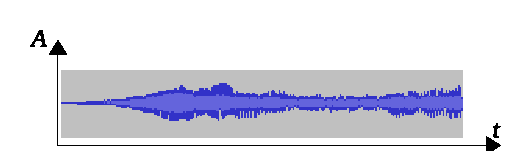
\includegraphics[width=0.8\textwidth]{resources/waveform-example.eps}
    \caption{Contoh representasi bentuk gelombang dari suara keluaran} \label{waveformexample}
\end{figure}

\begin{figure}[h]
    \centering
    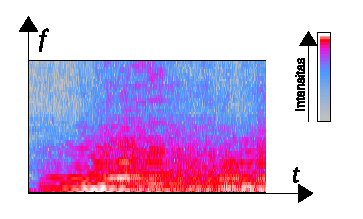
\includegraphics[width=0.8\textwidth]{resources/spectogram-example.eps}
    \caption{Contoh representasi spektogram dari suara keluaran} \label{spectogramexample}
\end{figure}

Komponen sistem ini dapat dibagi menjadi sistem perencana gestur dan pembangkit suara \parencite{Thippur2013ProbabilisticMO} seperti pada gambar \ref{thippurcomponents}. Keluaran dari sistem perencana gestur adalah rencana gestur ekspresif seperti keras-lemah suara, deskripsi timbre, deskripsi tempo, dan deskripsi teknik permainan spesifik alat musik. Komponen-komponen sistem ini dapat pula dipisahkan menjadi sistem perencana ekspresi, perencana gestur, dan pembangkit suara \parencite{yu2017bowing} seperti terlihat pada gambar \ref{yucomponents}. Perencana ekspresi bertugas membaca partitur dan menentukan rencana ekspresi dalam permainan tersebut. Contoh rencana ekspresi adalah \textit{espressivo} (ekspresif), \textit{scherzando} (melawak), \textit{tranquillo} (tenteram), dan sebagainya \parencite{yang2016synthesis}.

Suara yang dihasilkan dalam suatu permainan dipengaruhi oleh rencana gestur yang dieksekusi. Representasi rencana gestur dan informasi yang terkandung di dalamnya bergantung kepada jenis alat musik dan desain sistem. Spesifikasi energi tiap not, yang berhubungan dengan keras lemahnya not, lalu kepada alur perubahan dinamika sepanjang lagu, umum digunakan pada banyak alat musik. Spesifikasi energi di dalam not dan perubahannya sepanjang not mungkin hanya relevan untuk alat musik dengan eksitasi kontinu seperti alat gesek, alat tiup, dan nyanyian. Pada alat gesek, spesifikasi energi dan pilihan warna suara mungkin saja digantikan dengan spesifikasi cara menggesek (\textit{bowing}). Posisi \textit{bowing} dapat diubah, baik dari jarak dengan \textit{bridge} maupun pada bagian \textit{bow} mana senar tertempel. Begitu pula kecepatan dan tekanan \textit{bowing} dapat berpengaruh kepada \textit{timbre} dan dinamika. \parencite{yu2017bowing} Contoh gestur lainnya adalah \textit{vibrato}: naik turunnya \textit{pitch} (tinggi rendahnya frekuensi formant utama/\textit{f0}) dalam alat musik gesek atau naik turunnya amplitudo secara periodik dalam satu not. Gestur \textit{vibrato} mungkin saja sudah implisit terkandung dalam rencana realisasi \textit{pitch}. Dalam desain representasi rencana gestur, satu jenis gestur mungkin tidak digunakan karena sudah terkandung secara implisit dalam jenis gestur lain, data lain, atau bahkan mungkin pula diabaikan.

Dalam pembangunan CSEMP dan komponennya, pembagian ini tidak mutlak. Selain sistem yang membuat rencana-rencana ekspresi dan gestur terlebih dahulu sebelum dieksekusi menjadi suara, terdapat pula sistem yang langsung membangkitkan suara dari partitur tanpa adanya keluaran antara.

\begin{figure}[h]
    \centering
    \includegraphics[width=0.8\textwidth]{resources/CSEMP-Components-Thippur.eps}
    \caption{Komponen-komponen CSEMP berdasarkan \citet{Thippur2013ProbabilisticMO}} \label{thippurcomponents}
\end{figure}

\begin{figure}[h]
    \centering
    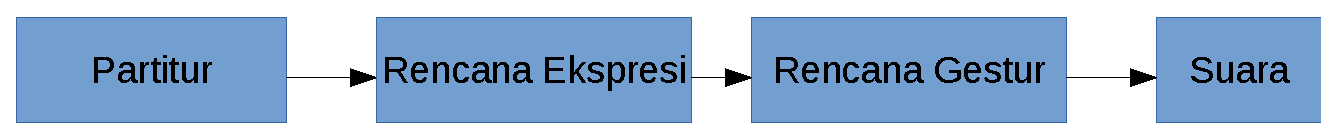
\includegraphics[width=0.8\textwidth]{resources/CSEMP-Components-Yu.eps}
    \caption{Komponen-komponen CSEMP berdasarkan \citet{yu2017bowing}}\label{yucomponents}
\end{figure}

\textit{Scope} dari penelitian-penelitian sebelumnya bermacam-macam. Terdapat sistem permainan music ekspresif yang bersifat \textit{end-to-end}, yaitu membangkitkan suara ekspresif dari masukan partitur. Penelitian bonada \parencite{bonada2017singing} membangkitkan suara vokal ekspresif dari partitur. Meski jangkauan konteks temporal yang dipertimbangkan dalam sistem Bonada hanya meliputi waktu yang dekat (dengan medan reseptif 100ms jaringan syaraf tiruan dengan konvousi terdilasi), suara yang dibangkitkan memiliki ekspresi dengan taraf tertentu. Suara yang dibangkitkan dengan sistem Bonada telah diujikan pula kepada pendengar manusia, meski belum mencapai taraf kealamian seperti pemain manusia.

Sistem lainnya yang telah mampu membangkitkan suara dari partitur saja (\textit{end-to-end}) adalah CaRo \parencite{canazza2015}. Untuk memainkan partitur dan membangkitkan suara, CaRo mengirimkan sinyal perintah permainan kepada mesin piano akustik. Dalam uji pendengar manusia \parencite{schubert2017test}, dibuktikan bahwa permainan CaRo tidak dapat dibedakan dari permainan manusia oleh pendengar manusia.

Terdapat penelitian lain yang hanya melingkupi sistem perencanaan gestur saja. Salah satunya adalah sistem perencanaan gestur untuk alat musik dengan eksitasi diskrit \parencite{miranda2010}. Ukuran kinerja dari sistem seperti ini hanya berupa akurasi dari data gestur ekspresi.

Terdapat penelitian lain yang hanya melingkupi sintesis suara saja. Nsynth \parencite{nsynth2017} mampu membangkitkan alat musik secara umum. Namun, suara yang dihasilkan hanya berupa suara satu not.

\section{Sistem Permainan dan Sintesis Musik Ekspresif Alat Musik Gesek}

Belum ada sistem permainan dan sintesis ekspresif untuk alat musik gesek yang mampu membangkitkan dari masukan partitur saja menjadi suara ekspresif. Telah ada penelitian-penelitian yang mengajukan komponen dari CSEMP untuk alat musik gesek.

Telah ada teknik sintesis yang mampu menghasilkan suara berbagai instrumen - termasuk alat musik gesek - dengan frasa yang natural, yaitu teknik \textit{Reconstructive Phrase Modeling} \parencite{lindemann2007rpm}. Input dari sistem ini adalah partitur dan gestur ekspresif. Gestur ekspresif yang menjadi masukan terdiri dari kontrol tiap not dan kontrol kontinu. Kontrol tiap not terdiri dari \textit{pitch} dan intensitas not. Kontrol kontinu terdiri dari intensitas \textit{vibrato}, tingkat keras instrumen, timbre, dan \textit{pitch-bend}. Keluaran dari sistem ini adalah prediksi harmonik, yang kemudian dapat langsung digunakan untuk sintesis suara.

Meski sudah dapat menghasilkan suara, penelitian \citet{lindemann2007rpm} masih membutuhkan masukan gestur ekspresif yang memiliki beberapa  masalah. Masalah pertama adalah format dari deskripsi gestur tidak didasarkan pada cara permainan alat musik gesek melainkan \textit{keyboard}. Masalah kedua, yang juga disebabkan masalah pertama, adalah besarnya kemungkinan kesalahan masukan gestur ekspresi baik pada data latih maupun pada pengujian/penggunaan sistem. Masalah lainnya adalah tidak tidak fleksibelnya keluaran yang dihasilkan, karena teknik \textit{Reconstructive Phrase Modeling} mencocokkan masukan dengan basis data frasa dan memainkan serupa dengan frasa yang telah ada di basis data.

Terdapat sistem lain yang membangkitkan \textit{waveform} secara langsung tanpa melalui prediksi harmonik. Nsynth \parencite{nsynth2017} mampu menghasilkan satu not saja. Meski suara yang dihasilkan diklaim berupa suara natural, namun karena yang dibangkitkan hanya satu not, sistem ini belum mampu membangkitkan suara musik dari partitur yang mengandung satu lagu lebih dari satu not secara ekspresif. Suara yang dihasilkan akan memiliki gestur ekspresi yang sama untuk setiap not.

Terdapat sistem serupa menghasilkan suara yang tidak mempertimbangkan konteks not \parencite{yang2016synthesis}. Namun, sistem ini mampu mempertimbangkan \textit{term} ekspresi musik yang diberikan sebagai input. Sistem ini mampu menghasilkan suara dengan manipulasi durasi, vibrato, dan dinamika. Pengujiannya dilakukan dengan kemiripan visual spektogram. Kekurangannya adalah di satu karya dengan satu ekspresi musik, not yang memiliki panjang sama akan diberi gestur yang sama.

Beberapa sistem lain hanya memberikan perencanaan gestur alat musik gesek. Terdapat sistem yang mampu memberikan rencana gestur untuk kuartet alat musik gesek. \parencite{marchini2014quartet} Sistem ini mampu membangkitkan rencana gestur berupa tingkat keras suara, kecepatan \textit{bow}, jangkauan \textit{vibrato}, dan perpanjangan not. Pengujian dalam penelitian tersebut hanya dilakukan terhadap satu kutipan karya yang sama dengan data latih dengan ukuran kinerja koefisien korelasi.

Terdapat sistem perencanaan gestur lainnya untuk alat musik violin dan viola \parencite{yu2017bowing}, namun gestur yang dihasilkan hanya berupa posisi \textit{bowing}. Sistem tersebut mampu menerima masukan partitur dan menghasilkan posisi \textit{bowing} tiap not seperenambelasan. Pengujian sistem ini telah dilakukan hanya terhadap satu kutipan karya dengan data latih berupa kutipan karya lain. Kinerja sistem ini diukur dengan koefisien korelasi dan akurasi.

Meski terdapat komponen-komponen CSEMP alat musik gesek, terdapat masalah dalam penggabungan komponen sistem yang telah ada. Pertama, output dari sistem yang telah ada bisa jadi tidak lengkap \parencite{yu2017bowing}. Kedua, sistem yang ada tidak kompatibel untuk langsung digabungkan. Input untuk sistem sintesis yang telah ada \parencite{lindemann2007rpm} menerima masukan dari pemain \textit{keyboard}. Sistem sintesis tersebut tidak mendukung masukan kecepatan \textit{bow} \parencite{marchini2014quartet}\parencite{yu2017bowing} dan posisi \textit{bow}\parencite{yu2017bowing}. Gestur \textit{vibrato} dalam alat musik gesek terdiri dari jangkauan dan kerapatan, sementara dalam masukan \textit{keyboard} disederhanakan menjadi intensitas saja.

Terdapat sebuah \textit{framework} CSEMP alat musik gesek untuk pembangkitan suara dari partitur non-expresif \parencite{perez2015} menggunakan pemodelan instrumen, pemain dan akustik. Namun, sistem ini hanya berupa \textit{framework} umum yang perlu didetilkan kembali. Selain itu, pemisahan pemodelan ini meniscayakan kebutuhan anotasi gestur secara manual.

\section{Sintesis Parametrik Neural} \label{literature-neural-parametric}

\citet{bonada2017singing} mengajukan sebuah teknik untuk sintesis suara nyanyian ekspresif. Ide dari teknik parametrik neural \parencite{bonada2017singing} adalah membangkitkan suara dalam representasi yang \textit{rate}-nya jauh lebih kecil dibandingkan dengan teknik WaveNet\parencite{Oord2016WaveNetAG} yang membangkitkan\textit{waveform} secara langsung, sehingga pembangkitan dapat berjalan lebih cepat. Dalam riset \citet{bonada2017singing}, representasi yang digunakan adalah parameter \textit{vocoder}. Suara nyanyian dibangkitkan oleh sebuah \textit{vocoder} dari parameter-parameter \textit{timing} fonetik, \textit{timbre}, dan \textit{pitch}. Parameter-parameter ini dibangkitkan dengan model \textit{timing} fonetik, model \textit{timbre}, dan model \textit{pitch} yang dilatih dengan data latih partitur non ekspresif dan suara nyanyian ekspresif. Arsitektur sistem ini tampak pada gambar \ref{fig-system-overview-bonada}.

\begin{figure}[h]
    \centering
    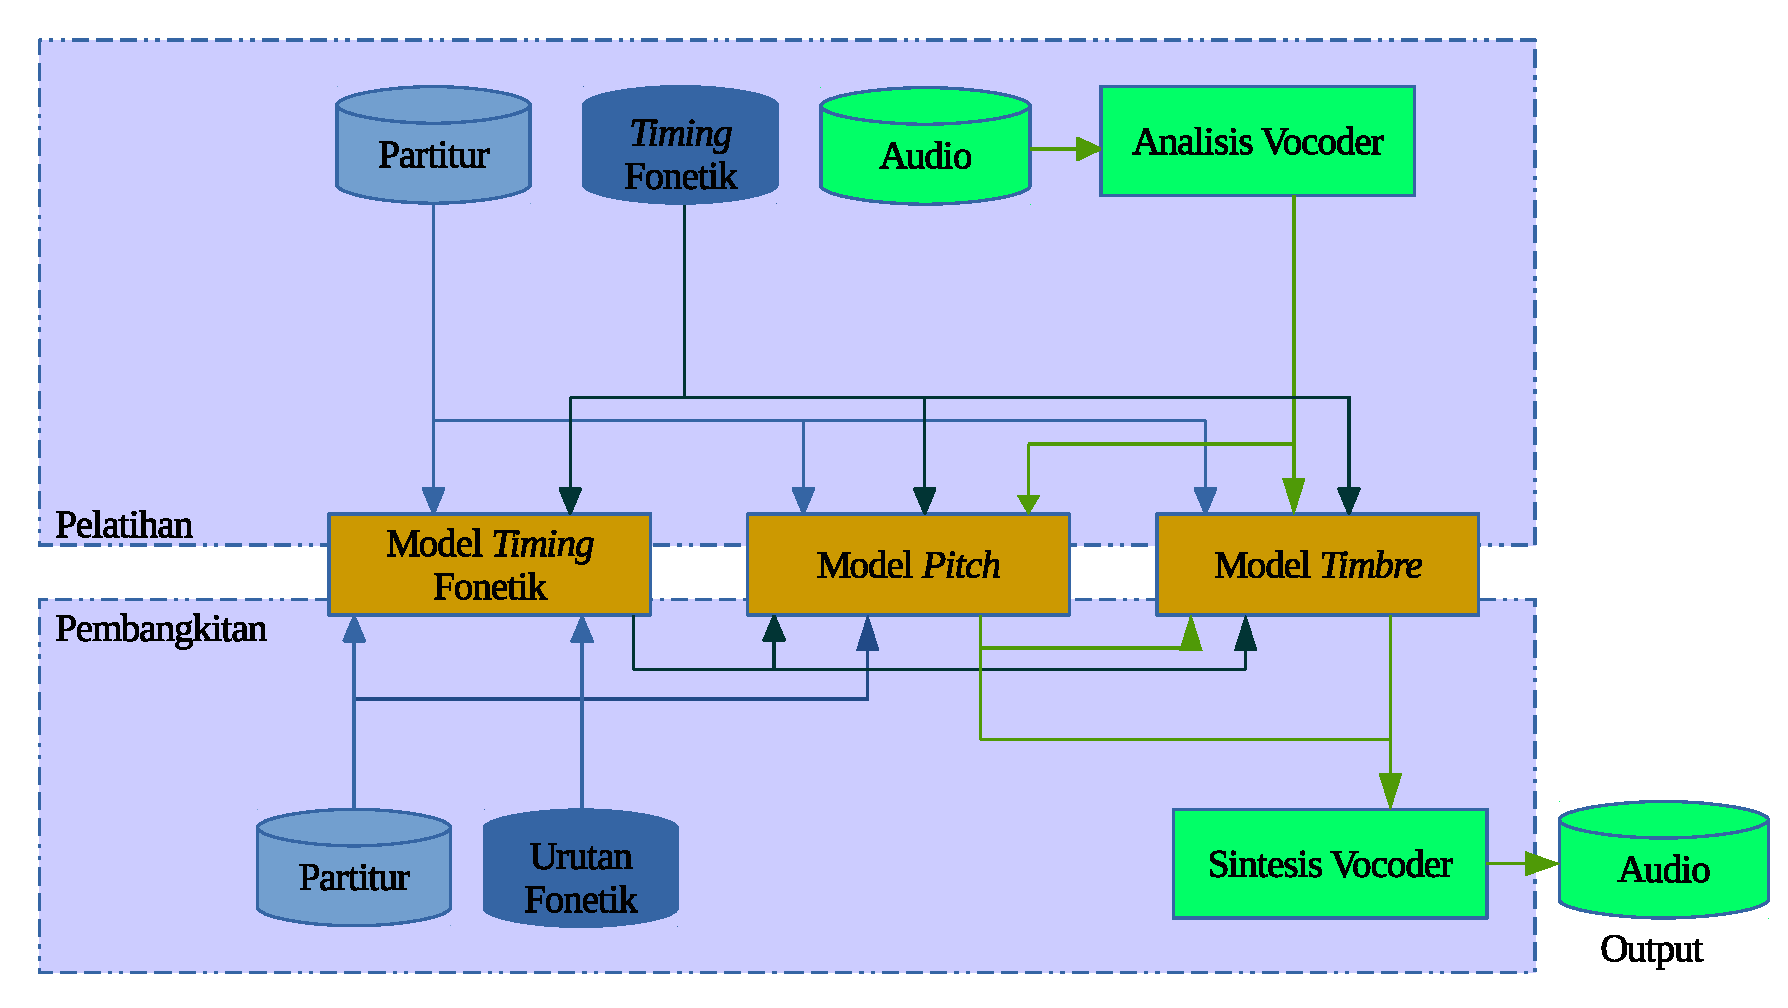
\includegraphics[width=0.8\textwidth]{resources/system-overview-bonada.eps}
    \caption{Arsitektur sistem sintesis parametrik neural untuk nyanyian \parencite{bonada2017singing}}\label{fig-system-overview-bonada}
\end{figure}

Dalam sistem ini, terdapat tiga model, yang menghasilkan parameter-parameter yang kemudian digunakan \textit{vocoder} untuk menghasilkan suara nyanyian ekspresif. Model-model ini dilatih menggunakan data latih berupa partitur, label \textit{timing} fonetik, dan rekaman nyanyian partitur yang bersesuaian oleh penyanyi profesional. Rekaman penyanyi dianalisis dengan vocoder untuk mendapatkan representasi \textit{pitch} dan \textit{timbre}. Masukan dan keluaran tiap model tercantum dalam tabel \ref{tab-models-in-out-bonada}. \ref{bonada2017singing}

\begin{table}[h]
	\centering
    \caption{Masukan dan Keluaran Tiap Model dalam Sistem Sintesis Parametrik Neural Suara Nyanyian \parencite{bonada2017singing}}\label{tab-models-in-out-bonada}
	\begin{tabular}{ |c|c|c| } 
	 \hline
	 Model & Masukan & Keluaran \\
	 \hline 
	 Model \textit{timing} & partitur & \textit{timing} (terdistorsi) not \\ 
	 fonetik  & urutan fonetik & \textit{timing} fonetik \\ 
	 \hline
	 Model \textit{pitch} & partitur & F0 \\ 
	  & \textit{timing} (terdistorsi) not  & \\ 
	 \hline
	 Model \textit{timbre} &  \textit{timing} fonetik\&not & V/UV \\ 
	  & F0 & Komponen harmonik\\ 
	  &   & Komponen aperiodisitas\\ 
	 \hline
	\end{tabular}
\end{table}

Untuk model \textit{timing} not, digunakan jaringan syaraf tiruan \textit{feedforward} dengan fitur kontekstual untuk tiap not dalam partitur. Untuk model \textit{durasi} fonem, digunakan jaringan syaraf tiruan konvolusional. \parencite{bonada2017singing} Untuk model \textit{pitch} dan model \textit{timbre}, digunakan jaringan syaraf tiruan dengan arsitektur yang didasarkan kepada WaveNet \parencite{Oord2016WaveNetAG}, yang tampak pada gambar \ref{fig-network-architecture-bonada}. \parencite{bonada2017singing}

\begin{figure}[h]
    \centering
    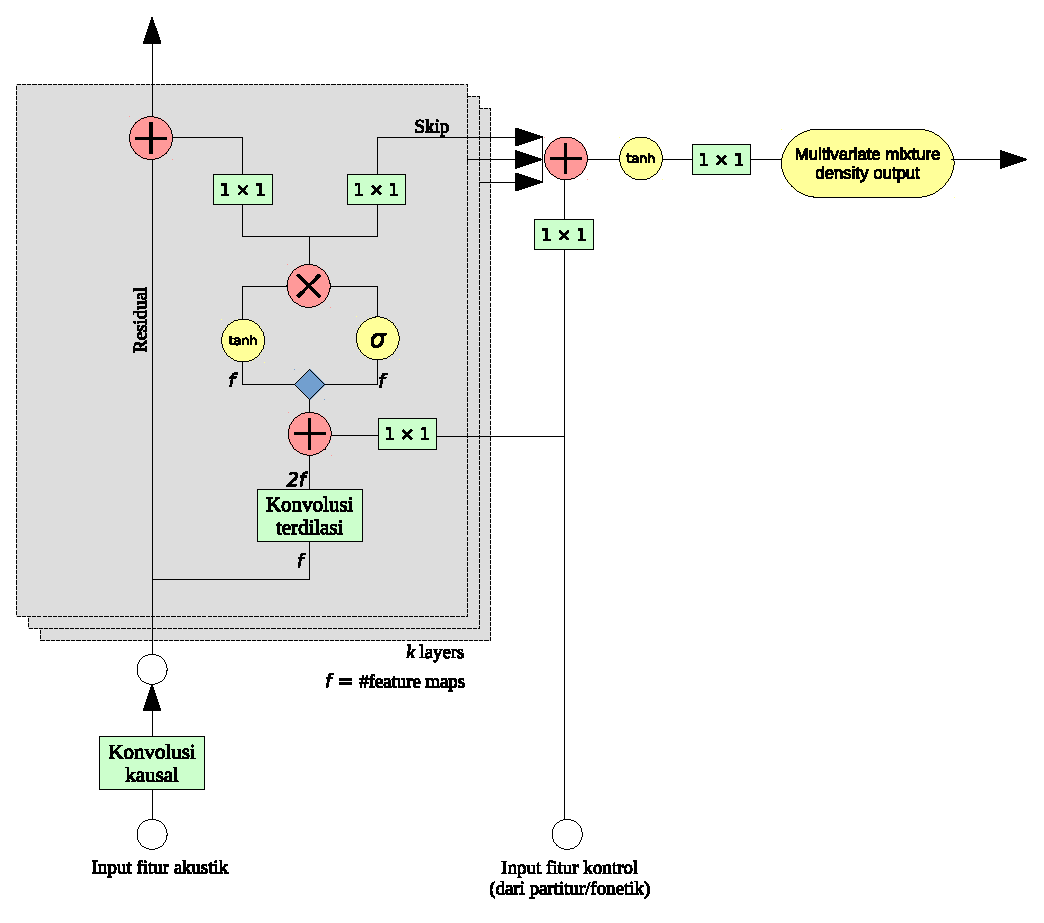
\includegraphics[width=0.8\textwidth]{resources/network-architecture-bonada.eps}
    \caption{Arsitektur jaringan syaraf tiruan modifikasi WaveNet yang digunakan pada sintesis neural parametrik untuk nyanyian\parencite{bonada2017singing}}\label{fig-network-architecture-bonada}
\end{figure}

Model ini menerima masukan fitur akustik dengan konvolusi kausal terdilasi \parencite{Oord2016WaveNetAG}, yang terlihat pada gambar \ref{fig-dilated-cnn}. Dengan demikian, model mampu mempertimbangkan keluaran-keluaran sebelumnya untuk memprediksi fitur akustik pada \textit{frame} selanjutnya. Medan reseptif konteks temporal dari jaringan syaraf tiruan ini, dengan konfigurasi pada riset \citet{bonada2017singing}, mencapai 100ms.

\begin{figure}[h]
    \centering
    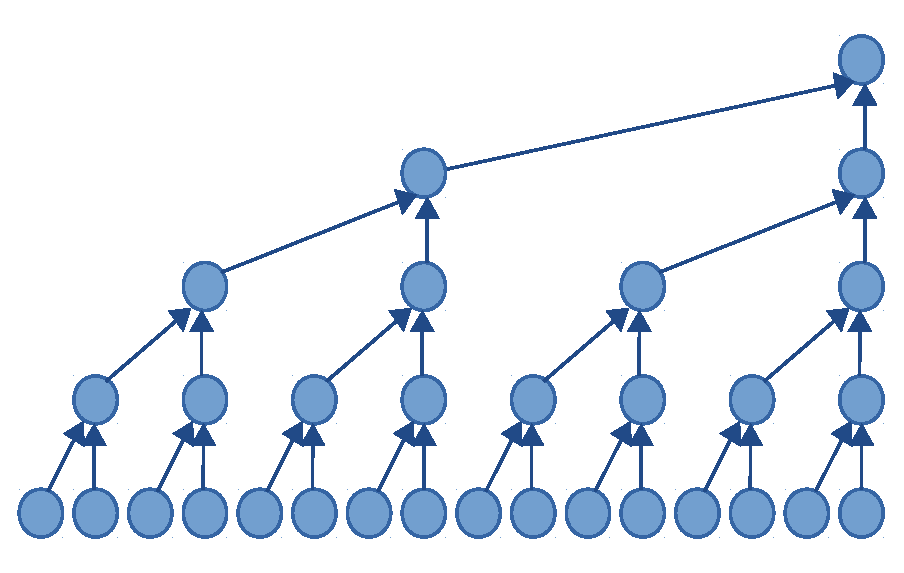
\includegraphics[width=0.8\textwidth]{resources/dilated-cnn.eps}
    \caption{Visualisasi tumpukan lapisan-lapisan konvolusi kausal terdilasi \parencite{Oord2016WaveNetAG}}\label{fig-dilated-cnn}
\end{figure}

Fitur akustik yang telah dilakukan konvolusi kausal terdilasi digabungkan dengan input fitur kontrol dari partitur dan fonetik. Setelah itu, unit aktivasi yang digunakan adalah unit aktivasi bergerbang \parencite{Oord2016ConditionalIG}. Dengan demikian, fungsi aktivasi yang diterapkan kepada masukan gabungan fitur-fitur akustik dan fitur-fitur kontrol menjadi:

\begin{equation}
    \mathbf{z} = tanh(W_{f,k}*\mathbf{x}+V^T_{f,k}\mathbf{h})\odot\sigma(W_{g,k}*\mathbf{x}+V^T_{f,k}\mathbf{h})
\end{equation}\label{eq-gated-activation}

dengan $*$ menunjukkan operator konvolusi, $\odot$ menunjukkan operasi perkalian tiap-elemen, $\sigma$ merupakan fungsi sigmoid, $k$ indeks lapisan, $f$ dan $g$ merupakan filter dan gerbang, $W$ dan $V$ adalah bobot konvolusi untuk masukan fitur akustik dan fitur kontrol yang dapat dipelajari.

Dari satu lapisan ke lapisan lain, diberikan koneksi residual. Serta, dari tiap lapisan, terdapat koneksi skip menuju lapisan output. Dengan cara ini, dapat dilatih jaringan syaraf tiruan yang memiliki lebih banyak lapisan. \parencite{He2016DeepRL}

Pada lapisan output, output tiap lapisan kembali dijumlahkan dengan masukan kontrol. Setelah itu, kembali dikenakan fungsi $tanh$\parencite{bonada2017singing}. Berbeda dengan WaveNet \parencite{Oord2016WaveNetAG} yang menggunakan distribusi keluaran SoftMax, pada teknik neural parametrik digunakan distribusi keluaran \textit{multivariate mixture density}. \textit{Mixture density} yang digunakan adalah Constrained Gaussian Mixture dengan $K=4$ Gaussian: \parencite{bonada2017singing}

\begin{equation}
    p(x) = \sum\limits_{k=0}^{K-1}w_k\mathcal{N}(x;\mu_k,\sigma_k^2)
\end{equation}\label{eq-gated-activation}

Dengan parameter-parameter $w_k$, $\mu_k$, $\sigma_k$ untuk $k=0,1,...,K-1$ dihitung dari empat parameter bebas: $\xi$, skala $\omega$, kemencengan $\alpha$, dan bentuk $\beta$. Bila jaringan memprediksi empat keluaran dengan aktivasi linear, $a_0$, $a_1$, $a_2$, $a_3$, parameter bebas ini diperoleh dengan cara sebagai berikut: \parencite{bonada2017singing}

\begin{equation}
    \xi = 2 sigm(a_0)-1; range[-1,1]
\end{equation}
\begin{equation}
    \omega = \dfrac{2}{255}e^{4sigm(a_1)}; range[\dfrac{2}{255}, \dfrac{2 e^4}{255}]
\end{equation}
\begin{equation}
    \alpha = 2 sigm(a_2)-1; range[-1,1]
\end{equation}
\begin{equation}
    \beta = 2 sigm(a_3); range[0,2]
\end{equation}

Kemudian, parameter-parameter Gaussian $w_k$, $\mu_k$, dan $\sigma_k$ dihitung sebagai berikut:\parencite{bonada2017singing}
\begin{equation}
    \sigma_k = \omega e^{(|\alpha|\gamma_s-1)k|}
\end{equation}
\begin{equation}
    \mu_k = \xi + \sum\limits_{i=0}^{k-1}\sigma_k\gamma_u\alpha
\end{equation}
\begin{equation}
    w_k = \dfrac{\alpha^{2k}\beta{k}\gamma_w^k}{\Sigma_{j=0}{K-1}\alpha^{2i}\beta{i}\gamma_w^i}
\end{equation}

dengan konstanta $\gamma_u$, $\gamma_s$, dan $\gamma_y$ di-$tune$ secara manual.

%\subsection{\textit{Vocoder} dan Pemodelan Spektral}

%Vocoder adalah ......

%Pemodelan spektral .....

%Model sinusoidal ...

%Nunggu dicoba dulu
    \chapter{Analisis dan Perancangan}

\section{Analisis Masalah}

Akan digunakan teknik parametrik neural untuk membangkitkan suara alat musik gesek. Untuk teknik ini, terdapat beberapa perbedaan masalah dengan penelitian sebelumnya\parencite{bonada2017singing}. Perbedaan masalah yang terjadi terdapat pada data input untuk sintesis, data latih, \textit{timing}, dan konteks.

Perbedaan masalah untuk data input sintesis terkait dengan \textit{timbre}. Dalam pembangkitan suara alat musik gesek, \textit{timbre} ditentukan oleh konteks. Hal ini berbeda dengan penelitian sebelumnya, di mana \textit{timbre} ditentukan dari rangkaian fonem yang terdapat dalam data input.

Perbedaan masalah terkait dengan data latih terdapat pada pewaktuan. Dalam penelitian ini, pewaktuan tidak terdapat pada data input.

\textit{Timing} not dalam alat musik gesek memiliki karakteristik yang berbeda dengan suara nyanyian. Dalam sistem baseline untuk suara nyanyian, terdapat \textit{timing} fonetik. Dalam sistem ini, tidak ada \textit{timing} fonetik. Hanya dibutuhkan \textit{timing} not saja.

Perbedaan masalah terkait konteks yaitu pada medan reseptif dari jaringan syaraf tiruan pada baseline. Baseline yang digunakan memiliki medan reseptif 100ms. Kecilnya medan reseptif ini berpengaruh kepada suara ekspresif secara umum, dan juga kepada penentuan \textit{timbre}. Untuk membangkitkan suara ekspresif, dibutuhkan konteks global dan konteks lokal dari not. Selain itu, konteks juga dibutuhkan dalam \textit{timbre}, yang dalam sintesis suara alat musik gesek tidak dipandu oleh rangkaian fonem.

\section{Rancangan Umum Sistem}

Untuk mengatasi masalah-masalah yang telah disebutkan, akan digunakan teknik neural parametrik serupa dengan baseline\parencite{bonada2017singing} dengan modifikasi. Modifikasi pertama yang diajukan adalah modifikasi pada arsitektur umum sistem. Modifikasi kedua yang diajukan dilakukan kepada arsitektur jaringan syaraf tiruan.

Arsitektur sistem yang diajukan terlihat pada gambar \ref{fig-system-overview}, sebagai modifikasi dari gambar \ref{fig-system-overview-bonada}. Dalam sistem ini, tidak ada masukan \textit{timing} fonetik untuk pelatihan. Partitur yang menjadi masukan pun tidak memiliki deskripsi fonem dan lirik. Model \textit{timing} fonetik diganti menjadi model \textit{timing}. Dalam sistem ini, ada komponen tambahan yaitu alignment dan analisis \textit{timing}.

Dalam sistem ini, \textit{timing} tidak diberikan dari data latih. Karenanya, \textit{timing} harus mampu diinferensi dari masukan partitur dan audio saja. Untuk inferensi \textit{timing} dari audio dan partitur, digunakan teknik alignment menggunakan masukan partitur dan hasil analisis vocoder dari audio. Hasil analisis vocoder yang digunakan adalah frekuensi fundamental dan kesunyian.

Berbeda dengan sistem baseline, model \textit{timbre} yang diajukan dalam sistem ini harus mampu menentukan \textit{timbre} dari konteks partitur. Karenanya, model \textit{timbre} dalam pelatihan menerima masukan partitur dan \textit{timing}, lalu dilatih untuk memprediksi data analisis vocoder. Parameter analisis vocoder yang diprediksi oleh model \textit{timbre} adalah spectral envelope dan komponen aperiodic.

Model \textit{timing} dalam sistem ini dilatih menggunakan partitur dan hasil analisis \textit{timing}. Dengan demikian, diharapkan model \textit{timing} dapat memprediksi \textit{timing} dari not dalam partitur.

Model pitch dalam sistem ini dilatih untuk menghasilkan F0. Masukan model ini adalah partitur dan \textit{timing}. Dalam pelatihan, masukan partitur diambil dari data latih, \textit{timing} diambil dari hasil alignment dan analisis \textit{timing}, dan parameter vocoder diambil dari hasil analisis vocoder terhadap audio.

Dengan demikian, terdapat tiga model, yaitu model \textit{timing}, \textit{pitch}, dan \textit{timbre}. Masukan dan keluaran tiap-tiap model ini tertulis dalam tabel \ref{tab-models-in-out}. Terdapat dua perbedaan dari masukan dan keluaran model-model baseline pada tabel \ref{tab-models-in-out-bonada}. Pertama, tidak ada fonetik. Kedua, model \textit{timbre} menerima masukan partitur.

\begin{table}[h]
    \centering
    \caption{Masukan dan Keluaran Tiap Model dalam Sistem Sintesis Parametrik Neural Suara Alat Musik Gesek }\label{tab-models-in-out}
    \begin{tabular}{ |c|c|c| } 
     \hline
     Model & Masukan & Keluaran \\
     \hline 
     Model \textit{timing} & partitur & \textit{timing} not (dengan penyimpangan) \\ 
     \hline
     Model \textit{pitch} & partitur & F0 \\ 
      & \textit{timing} (terdistorsi) not  & \\ 
     \hline
     Model \textit{timbre} & partitur & V/UV \\ 
      & \textit{timing} (terdistorsi not)  & Komponen harmonik\\ 
      & F0  & Komponen aperiodisitas\\ 
     \hline
    \end{tabular}
\end{table}

\begin{figure}[h]
    \centering
    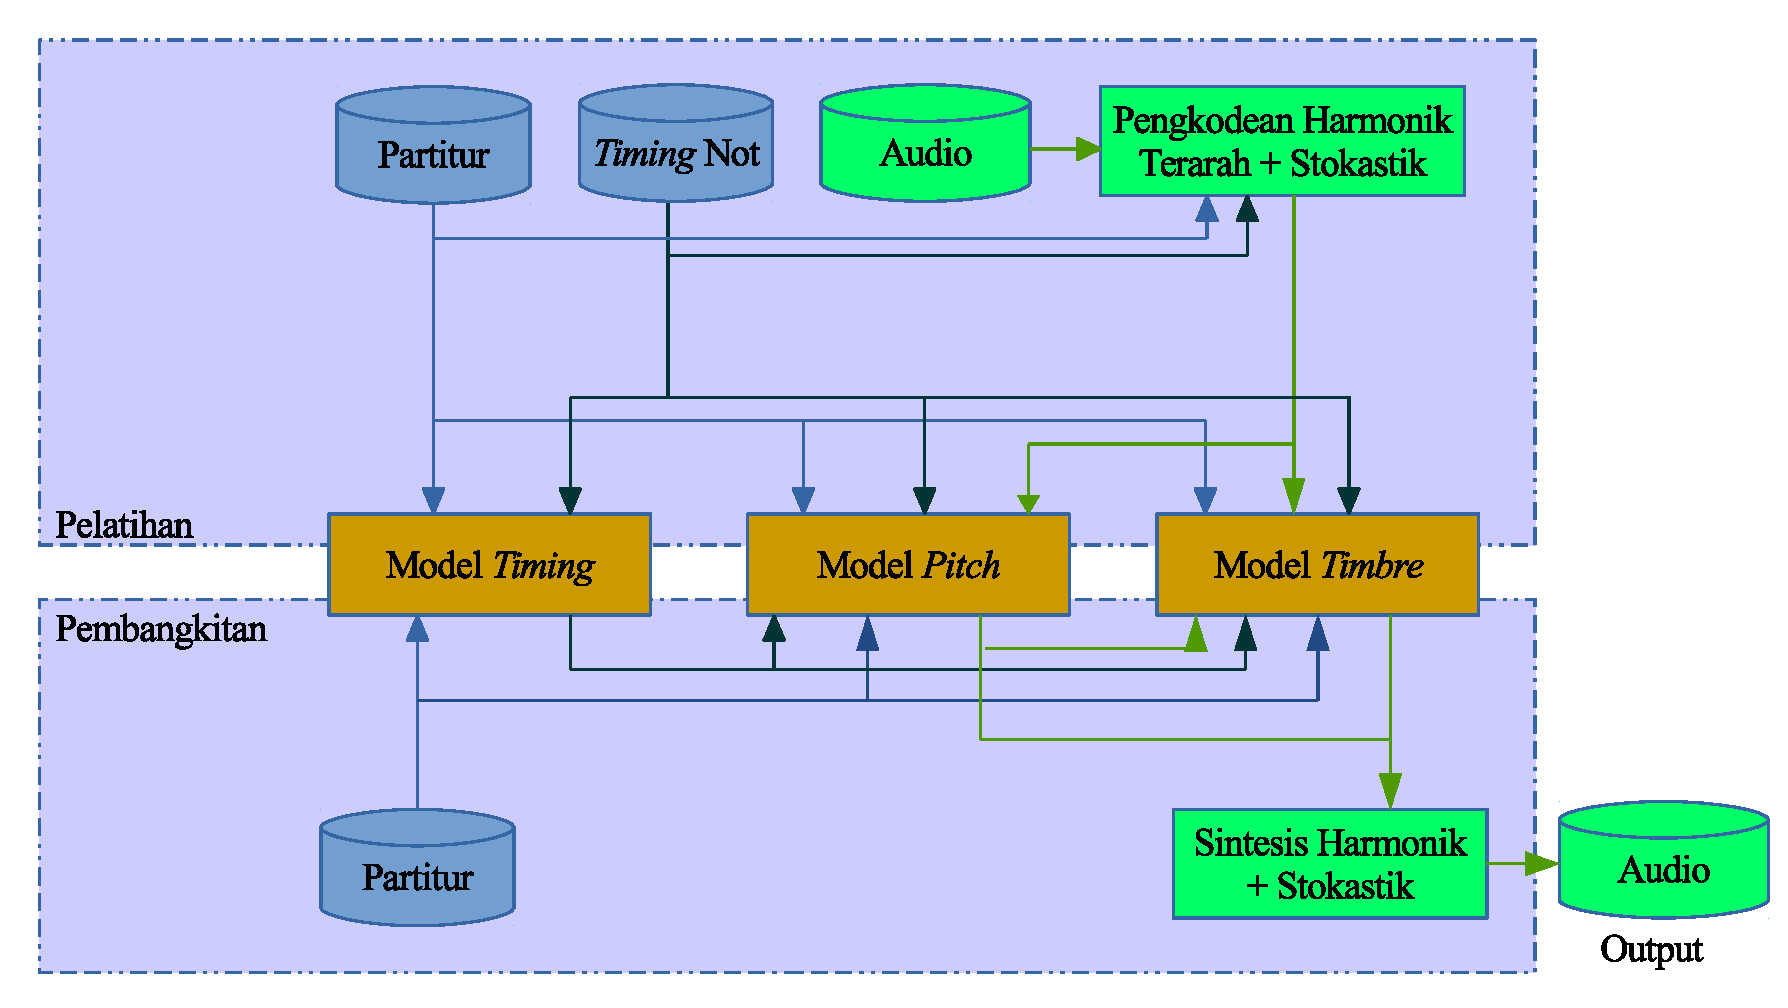
\includegraphics[width=0.8\textwidth]{resources/system-overview.eps}
    \caption{Arsitektur sistem permainan musik ekspresif alat musik gesek yang diajukan (modifikasi gambar \ref{fig-system-overview-bonada})}\label{fig-system-overview}
\end{figure}

Pada tahap pembangkitan, sistem ini mampu menerima partitur dan menghasilkan audio. Keluaran perantara yang dihasilkan adalah parameter vocoder, yang kemudian digunakan oleh vocoder untuk menghasilkan audio.

Hal pertama yang dilakukan dalam tahap pembangkitan adalah prediksi \textit{timing} not. Setelah itu, partitur dan \textit{timing} not digunakan untuk memprediksi pitch an \textit{timbre}, dengan model yang sesuai. Parameter pitch -frekuensi fundamental- dan parameter \textit{timbre} -spectral envelope dan aperiodisitas- digunakan untuk sintesis vocoder.

Tiap model dari model-model ini adalah model regresi. Untuk model \textit{timing}, digunakan jaringan syaraf tiruan \textit{feedforward}. Untuk model \textit{pitch} dan model \textit{timbre}, digunakan jaringan syaraf tiruan konvolusional terdilasi dengan elemen rekuren. Masukan dari jaringan syaraf tiruan ini terdiri dari masukan rekuren -output pada waktu sebelumnya- dan masukan kontrol.

Masukan kontrol jaringan syaraf tiruan ini berasal dari partitur dan dari \textit{timing}. Untuk model \textit{timing}, masukan kontrol hanya berasal dari partitur. Untuk model pitch dan model \textit{timbre}, masukan kontrol berasal dari partitur dan berasal dari \textit{timing}.

Masukan dari partitur dapat menunjukkan kondisi sesaat dan konteks. Kondisi sesaat berupa pitch asli, panjang not, dan waktu dalam not. Kondisi konteks dapat berupa not sebelum dan sesudah, interval, ataupun kondisi-kondisi lainnya hasil analisis karya. Namun, kakas analisis karya mungkin tidak akan digunakan karena riset terkait analisis karya menggunakan komputer masih minim.

\begin{figure}[h]
    \centering
    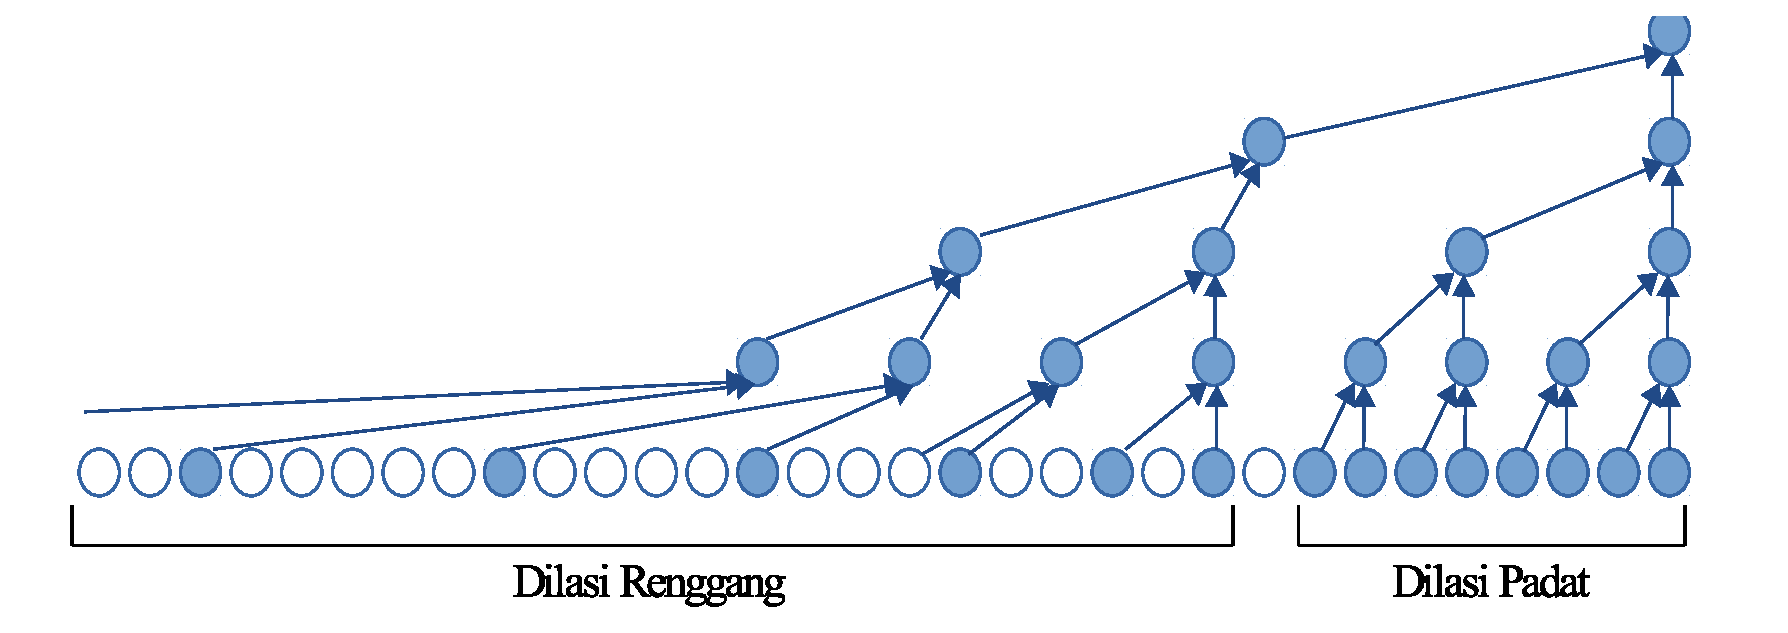
\includegraphics[width=0.8\textwidth]{resources/sparse-dense-dilated-cnn.eps}
    \caption{Arsitektur jaringan syaraf tiruan konvolusional dengan dilasi jarang-padat (modifikasi arsitektur pada gambar \ref{fig-dilated-cnn})}\label{fig-sparsedilated-cnn}
\end{figure}

Untuk mengatasi masalah medan reseptif dari model baseline, diajukan dilasi jarang-padat. Arsitektur jaringan syaraf tiruan yang merupakan modifikasi arsitektur pada gambar \ref{fig-dilated-cnn} terlihat pada gambar \ref{fig-sparsedilated-cnn}. Untuk simpul-simpul masukan yang dekat dengan frame yang sedang dibangkitkan, digunakan faktor dilasi sedemikian hingga semua simpul terlingkupi. Untuk simpul-simpul masukan yang jauh dari frame yang sedang dibangkitkan, digunakan faktor dilasi yang lebih besar. Dengan demikian, medan reseptif dapat ditingkatkan tanpa menambah jumlah simpul tersembunyi dan ukuran vektor bobot yang diestimasi.

Pada bagian dengan dilasi jarang, ada simpul-simpul yang dilewat. Dalam permasalahan suara alat musik gesek, hal ini tidak menjadi masalah. Karakteristik suara yang menjadi masukan rekuren banyak redundan. Adapun masukan kontrol untuk simpul-simpul yang berdekatan akan sama karena satu not dapat menjadi banyak frame di mana tiap frame menjadi simpul masukan.

Untuk melatih sistem ini, dibutuhkan data latih berupa partitur dan rekaman audio. Data yang dibutuhkan adalah data berpasangan. Detil pengumpulan data latih ini dijelaskan dalam subbab selanjutnya.

\section{Tahapan Pembangunan Sistem}

Terdapat empat tahapan pembangunan sistem:

\begin{enumerate}
    \item Pengumpulan data
    \item Implementasi program untuk pelatihan dan pembangkitan
    \item Pelatihan model
    \item Pengujian
\end{enumerate}

Pada tahap pengumpulan data yang dibutuhkan berupa data latih dan data uji. Dalam pengumpulan, data akan dihimpun menjadi satu kumpulan data. Kumpulan data tersebut akan dipisahkan menjadi data latih dan data uji setelah pengumpulan data selesai.

Untuk pengumpulan data, akan dicari partitur dan rekaman audio yang telah terpublikasi. Akan disaring instans data yang memiliki pasangan yang sesuai. Data rekaman audio tanpa partitur atau data partitur tanpa audio tidak akan dimasukkan kepada kumpulan data akhir. Kemudian, penyalin akan mendengarkan rekaman audio dan mencocokkan dengan partitur untuk memastikan bahwa rekaman audio sesuai dengan partitur. Partitur yang dikumpulkan akan disalin/dikonversi menjadi format teks (MusicXML/MIDI).

Karena pengujian yang akan dilakukan adalah pengujian pendengar manusia, data uji yang dibutuhkan berukuran kecil. Pemisahan data uji dari data latih dilakukan secara acak. Data uji akan diambil sejumlah 3-5 karya.

Implementasi program untuk pelatihan dan pembangkitan dilakukan menggunakan kakas-kakas \textit{vocoder} dan jaringan syaraf tiruan. Kakas jaringan syaraf tiruan yang digunakan adalah kakas yang mendukung jaringan syaraf tiruan \textit{feedforward}, konvolusi, dilasi, dan elemen rekuren. Hasil implementasi ini dapat digunakan untuk melatih model, yang kemudian digunakan untuk membangkitkan suara untuk diujikan kepada pendengar manusia.
    \chapter{Eksperimen Sistem Permainan Musik Ekspresif untuk Alat Musik Gesek}

\section{Tujuan Eksperimen}

Eksperimen dilakukan untuk menunjukkan kinerja sistem permainan musik ekspresif untuk alat musik gesek yang telah dibangun. Sistem permainan musik ekspresif diimplementasi berdasarkan hasil perancangan pada Bab \ref{design-chapter}. Kinerja yang akan diukur adalah kealamian ekspresi hasil sintesis suara oleh sistem tersebut. Kealamian memiliki makna seberapa mirip ekspresi pada permainan yang dihasilkan terhadap ekspresi permainan manusia.

Meski tujuan utama eksperimen ini adalah menunjukkan kinerja sistem utuh, eksperimen juga dilakukan lebih detil untuk mengetahui kinerja komponen dan teknik yang digunakan. Secara ringkas, hal-hal yang diujikan tertulis dalam Tabel \ref{tab-experiment-list}.

Sebelum pengujian untuk menunjukkan kinerja sistem permainan musik ekspresif untuk alat musik gesek, dilakukan eksperimen penyetelan parameter untuk menentukan parameter-parameter terbaik. Hal ini karena arsitektur model dan pelatihannya dipengaruhi oleh berbagai parameter.

Selain itu, dilakukan juga pengujian untuk membuktikan bahwa skema pemilihan subset data latih yang diuraikan dalam Subbab \ref{subsetselectionsection} mampu menghasilkan model dengan kinerja lebih baik daripada model yang dilatih langsung menggunakan keseluruhan data latih untuk model-model yang menggunakan arsitektur Wavenet yang dimodifikasi. Hal ini akan dibuktikan untuk model-model \textit{pitch} dan \textit{timbre}. Adapun untuk model \textit{timing}, dilakukan pengujian untuk membuktikan bahwa skema pemilihan subset data latih tidak menghasilkan model dengan kinerja yang lebih baik daripada model yang dilatih langsung menggunakan keseluruhan data latih.

\begin{table}[htbp]
    \centering
    \caption{Tujuan eksperimen yang dilakukan}\label{tab-experiment-list}
    \begin{tabular}{ |p{0.2\textwidth}|p{0.325\textwidth}|p{0.325\textwidth}|p{0.15\textwidth}| }
    \hline
    &\textbf{Tujuan}&\textbf{Hipotesis}&\textbf{Metrik}\\\hline
    \multicolumn{4}{|p{\textwidth}|}{Eksperimen komponen}\\\hline
    Penyetelan parameter&Menentukan parameter terbaik&-&Koefisien korelasi\\\hline
    Uji pemilihan subset&Membuktikan hipotesis&
    - Model \text{pitch} dan \textit{timbre}: kinerja dengan pemilihan subset $>$ kinerja tanpa pemilihan subset&Koefisien korelasi \\
    && - model \text{textit}: kinerja dengan pemilihan subset $<$ kinerja tanpa pemilihan subset& \\hline
    Uji korelasi komponen&Mengetahui kinerja masing-masing komponen & - & koefisien korelasi \\\hline
    \multicolumn{4}{|p{\textwidth}|}{Eksperimen sistem utuh}\\\hline
    Uji korelasi sistem utuh&Membuktikan hipotesis & Kinerja teknik yang diajukan $>$ kinerja korelasi teknik \textit{baseline}& Koefisien korelasi\\\hline
    Uji preferensi kealamian&Membuktikan hipotesis & Pendengar manusia menganggap permainan dari sistem yang diajukan lebih alami daripada sistem \textit{baseline}& Preferensi kealamian subjektif \\\hline
    \end{tabular}
\end{table}

\section{Skenario Eksperimen}
Eksperimen dilakukan untuk menilai tingkat kealamian dari ekspresi permainan musik yang dihasilkan. Penilaian dilakukan dengan uji korelasi dan uji persepsi kealamian pendengar.

Eksperimen diawali dengan eksperimen komponen sistem untuk menyetel parameter dan menguji korelasi tiap-tiap model yang menjadi komponen dari sistem ini. Setelah itu, eksperimen dilakukan dengan eksperimen uji korelasi sistem utuh.

Pada eksperimen komponen, model-model \textit{timing}, \textit{pitch} yang terdiri dari model deviasi f0, dan \textit{timbre} yang terdiri dari model frekuensi harmonik, magnitudo harmonik, serta amplop stokastik disetel parameternya dan diuji korelasinya.

Untuk penyetelan parameter model-model, dilakukan validasi silang dengan $k=5$. Berikut ini adalah langkah-langkah validasi silang:
\begin{enumerate}
	\item data dibagi menjadi $k$ bagian
	\item untuk tiap bagian, gunakan bagian tersebut untuk memvalidasi model yang dilatih dengan komplemennya
	\item rata-ratakan metrik kinerja terhadap semua bagian tersebut
\end{enumerate}

Parameter-parameter model yang disetel berbeda-beda untuk tiap modelnya. Untuk model \textit{timing}, sebelum penyetelan parameter, dilakukan pemilihan teknik antara ANN dan regresi DT. Setelah itu, apabila teknik yang terpilih adalah DT, parameter yang disetel adalah jumlah not konteks yang menjadi fitur dan kedalaman maksimum.

Untuk model-model f0, frekuensi harmonik, magnitudo harmonik, dan amplop stokastik, terdapat empat kelompok parameter:
\begin{itemize}
	\item parameter-parameter yang diambil dari riset neural parametrik nyanyian, yaitu:
	\begin{itemize}
		\item ukuran konvolusi kausal awal
		\item ukuran kanal residual
		\item ukuran konvolusi terdilasi
		\item ukuran \textit{batch}
		\item jumlah \textit{frame} keluaran \textit{valid}
		\item \textit{learning rate} (awal, \textit{decay}, interval)
	\end{itemize}
	\item parameter-parameter yang bukan dari riset neural parametrik nyanyian, namun tidak disetel dengan validasi silang, yaitu:
	\begin{itemize}
		\item \textit{output stage}: tetap CGM, namun dimensi disesuaikan
		\item temperatur pembangkitan $\tau$: bilangan kecil, dimensi disesuaikan
		\item Jumlah \textit{epoch}: sedikit di atas jumlah epoch pada neural parametrik nyanyian, namun dibatasi dengan \textit{early stopping}
	\end{itemize}
	\item parameter yang disetel dengan validasi silang, yaitu:
	\begin{itemize}
		\item faktor dilasi
		\item tingkat \textit{noise} pada masukan $\lambda$
		\item \textit{early stopping patience}
	\end{itemize}
	\item parameter terikat, berubah apabila faktor dilasi dan ukuran konvolusi berubah, yaitu:
	\begin{itemize}
		\item jumlah lapisan
		\item jumlah lapisan per \textit{stage}
		\item medan reseptif
	\end{itemize}
\end{itemize}

Untuk model f0, parameter yang diambil dari riset neural parametrik nyanyian diambil dari model f0 pada riset neural parametrik nyanyian. Untuk model frekuensi harmonik dan model magnitudo harmonik, parameter disesuaikan dari model amplop harmonik pada riset neural parametrik nyanyian. Untuk model amplop stokastik, parameter disesuaikan dari model aperiodisitas pada riset neural parametrik nyanyian.

Setelah parameter telah disetel, model dilatih dengan keseluruhan data latih. Namun, model ini tidak langsung diujikan terhadap data uji. Kinerja model ini dibandingkan terlebih dahulu dengan kinerja model yang telah dilatih pada tahapan validasi silang. Hal ini dilakukan untuk memilih model terbaik, karena mungkin saja model yang dilatih dengan data latih lebih besar memiliki kinerja yang lebih buruk. Hal ini dilakukan untuk model \textit{pitch} dan model \textit{timbre}. Adapun untuk model \textit{timing} akan digunakan model yang dilatih dengan keseluruhan data latih. Setelah dipilih model yang terbaik terhadap data latih, model diujikan terhadap data uji.

Validasi, pengujian, dan pengukuran kinerja tiap-tiap model dilakukan sesuai dengan masukan dan keluaran model-model tersebut. Model \textit{timing} diberi masukan partitur dan divalidasi \textit{timing} hasilnya. Model f0 diberi masukan partitur dan \textit{timing} dan divalidasi f0 hasilnya. Demikian pula, serupa pada model frekuensi harmonik, magnitudo harmonik, hingga amplop stokastik.

%TODO koefisien korelasi Pearson yang dituliskan pada Persamaan \ref{pearson-corrcoef-eq}
Metrik yang digunakan adalah koefisien korelasi Pearson. Untuk model-model f0, frekuensi harmonik, magnitudo harmonik, dan amplop stokastik, koefisien korelasi dihitung pasangan nilai-nilai pada keluaran dan nilai-nilai pada data tiap \textit{frame}. Untuk model \textit{timing}, koefisien korelasi dihitung terhadap nilai nada, dalam skala nomor not midi, untuk tiap \textit{frame} berdasarkan \textit{timing} yang dihasilkan, berpasangan dengan nilai nada berdasarkan \textit{timing} data.

Model-model dengan parameter yang telah disetel dan dilatih dalam tahapan eksperimen komponen kemudian digabungkan untuk membentuk sistem utuh. Setelah itu, sistem utuh digunakan untuk membangkitkan suara dengan masukan partitur pada data uji. Keluaran akhirnya --sebelum diubah menjadi sinyal gelombang-- berupa frekuensi harmonik, magnitudo harmonik, serta amplop stokastik divalidasi dengan frekuensi harmonik, magnitudo harmonik, serta amplom stokastik pada data uji.

Pada bagian terakhir eksperimen, yaitu uji persepsi, dilakukan pengujian kepada sejumlah responden. Sebelum dilakukan uji pendengaran, ditanyakan kepada responden data pengalaman responden terkait musik. Pada uji pendengaran, responden diberikan 9 pasang segmen audio. Tiap pasang terdiri dari 10 detik segmen keluaran sistem yang telah dibangun dan 10 detik segmen keluaran sistem \textit{baseline}.

Sistem yang dijadikan \textit{baseline} sebagai perbandingan adalah sistem Synful RPM. Untuk menghasilkan suara ekspresif, seharusnya sistem ini diberikan masukan partitur ekspresif. Namun, sebagai \textit{baseline} terhadap sistem yang dibangun, sistem ini diberi masukan yang sama dengan sistem yang telah dibangun yaitu partitur tanpa ekspresi.

Yang diuji dengan uji persepsi adalah sistem dengan teknik neural parametrik sebagai sistem permainan musik ekspresif partitur-ke-suara dan sebagai sistem perencana gestur ekspresi. Sebagai sistem permainan musik ekspresif partitur-ke-suara, suara keluaran sistem ini yang diperdengarkan kepada pendengar bersama dengan suara keluaran RPM tanpa masukan gestur ekspresi untuk dibandingkan. Sebagai sistem perencana gestur ekspresi, keluaran sistem dengan teknik neural parametrik yang dikonversi menjadi partitur ekspresif dijadikan masukan kepada sistem RPM, dan diperdengarkan kepada pendengar bersama dengan suara keluaran RPM tanpa gestur ekspresi untuk dibandingkan. Dengan demikian, tiap pendengar akan mendengarkan 9 pasang keluaran sistem Neural Parametrik dan RPM tanpa gestur serta 9 pasang keluaran RPM dengan gestur dari sistem Neural Parametrik dan RPM tanpa gestur. Dengan demikian, tiap pendengar mendengarkan 18 pasang segmen suara.

\begin{figure}
\centering
    \includegraphics[width=0.8\textwidth]{resources/questionnaire_screenshot.png}
    \caption{Tampilan cuplikan kuesioner yang digunakan untuk uji preferensi kealamian}\label{fig-questionnaire-sample}
\end{figure}

Urutan pasangan segmen-segmen ini diacak, kemudian urutan segmen tiap pasang juga diacak. Untuk tiap pasang, responden diminta untuk memilih segmen audio yang lebih alami. Dari hasil ini, dapat dihitung persentase preferensi sistem ini terhadap sistem \textit{baseline}. Selain itu, responden juga dapat menyebutkan pertimbangan memilih segmen suara tersebut. Responden dapat memilih pertimbangan dari daftar yang telah ada ataupun menuliskan pertimbangan baru. Cuplikan kuesioner yang digunakan dapat dilihat pada Gambar \ref{fig-questionnaire-sample}. %TODO Mean Preference Score dibenerin

\section{Hasil Eksperimen Komponen Sistem}

Hasil eksperimen komponen sistem terdiri dari eksperimen model \textit{timing}, \textit{pitch} yang terdiri dari model deviasi f0, dan \textit{timbre} yang terdiri dari model frekuensi harmonik, magnitudo harmonik, serta amplop stokastik. Eksperimen tiap-tiap model terdiri dari penyetelan parameter dan pengujian.

\subsection{Hasil penyetelan parameter}

Eksperimen model \textit{timing} dimulai dengan pemilihan teknik menggunakan validasi silang. Sebagaimana tampak pada Tabel \ref{tab-timing-model-tuning-results}, tampak bahwa teknik \textit{decision tree regression} memiliki kinerja yang lebih baik daripada ANN. Analisis lebih lanjut terhadap \textit{output} ANN tersebut menunjukkan bahwa deviasi \textit{timing} yang dihasilkan ANN adalah konstan. Hal ini menunjukkan bahwa ANN tidak dapat mempelajari pola deviasi \textit{timing} pada data latih.

\begin{table}[htbp]
    \centering
    \caption{Hasil validasi silang untuk penyetelan parameter model \textit{timing}}\label{tab-timing-model-tuning-results}
    \begin{tabular}{ |l|r| } 
     \hline
     Parameter & Pearson r untuk Nada Tiap \textit{Frame} \\
     \hline 
     \multicolumn{2}{|l|}{model regresi}\\ \hline
	 ann    &-0.03684115\\ \hline
	 dt, konteks=10, kedalaman=300     & 0.09796566\\ \hline
	 \multicolumn{2}{|l|}{penyetelan jumlah not konteks fitur}\\ \hline
	 dt, konteks=20, kedalaman=300       &0.07746795\\ \hline
	 dt, konteks=10, kedalaman=300      &0.09796566\\ \hline
	 dt, konteks=5, kedalaman=300     &0.14187831\\ \hline
	 dt, konteks=3, kedalaman=300     &\textbf{0.16475536}\\ \hline
	 dt, konteks=1, kedalaman=300      &0.10598458\\ \hline
	 \multicolumn{2}{|l|}{penyetelan kedalaman pohon}\\ \hline
	 dt, konteks=3, kedalaman=25 	 &0.15163629\\\hline
	 dt, konteks=3, kedalaman=50     &0.1326507\\\hline
	 dt, konteks=3, kedalaman=100      &0.12941929\\\hline
	 dt, konteks=3, kedalaman=300     &\textbf{0.16475536}\\ \hline
	 dt, konteks=3, kedalaman=600     &0.11958923\\\hline
	 dt, konteks=3, kedalaman=1000     &0.1351192   \\  \hline
    \end{tabular}
\end{table}

Hasil penyetelan parameter jumlah not konteks fitur dan kedalaman pohon juga terdapat pada Tabel \ref{tab-timing-model-tuning-results}. Parameter terbaik diperoleh dengan 3 not konteks fitur dan kedalaman pohon 300.

Penyetelan model berikutnya adalah penyetelan model f0. Tabel \ref{tab-f0-model-tuning-results} menunjukkan hasil validasi silang untuk penyetelan parameter model f0, dengan metrik berupa koefisien korelasi Pearson dari frekuensi fundamental hasil pembangkitan terhadap frekuensi fundamental pada data. Faktor dilasi yang menghasilkan kinerja terbaik adalah $1,2,4,8,16,32,1,2,4,8,16$. Faktor dilasi ini memiliki medan reseptif terhadap output sebelum yang lebih pendek daripada faktor dilasi pada riset neural parametrik nyanyian. Adapun tingkat \textit{noise} $\lambda$ terbaik didapatkan dengan nilai $0.4$, sama dengan pada riset neural parametrik nyanyian.

Pelatihan model f0 dengan \textit{early stopping} memiliki kinerja yang sama dengan pelatihan tanpa \textit{early stopping}. Hal ini karena dengan \textit{patience} 100, \textit{early stopping} tidak menghentikan pelatihan hingga jumlah \textit{epoch} maksimal yang bernilai 300. Karenanya, tanpa \textit{early stopping} ataupun dengan \textit{early stopping}, model f0 ini tetap dilatih dengan 300 \textit{epoch}.

\begin{table}[htbp]
    \centering
    \caption{Hasil validasi silang untuk penyetelan parameter model f0}\label{tab-f0-model-tuning-results}
    \begin{tabular}{ |l|l|l|r| } 
     \hline
     \multicolumn{3}{|l|}{Parameter} & Pearson r\\
     \cline{1-3}
     faktor dilasi & $\lambda$ & \textit{patience} & F0\\
     \hline 
	1,2,4,8,16,32,64,1,2,4,8,16,32 & 0.4 &100      &0.9525\\\hline
	1,2,4,8,16,32,1,2,4,8,16 & 0.4 &100            &0.9526\\\hline
	1,2,4,8,16,32,64,1,2,4,8,16,32 & 0.01 &100     &0.9516\\\hline
	1,2,4,8,16,32,1,2,4,8,16 & 0.01 &100           &0.9507\\\hline
	1,2,4,8,16,32,1,2,4,8,16 & 0.4 &tanpa \textit{early stopping}    &0.9526\\\hline
    \end{tabular}
\end{table}

Hasil penyetelan parameter model frekuensi harmonik tampak pada Tabel \ref{tab-freq-model-tuning-results}. Faktor dilasi yang memiliki kinerja terbaik adalah $1,2,4,1,2$, sama dengan pada riset sintesis neural parametrik nyanyian. Tingkat \textit{noise} $\lambda$ terbaik adalah $0.4$, sama dengan pada riset sintesis neural parametrik nyanyian. Model yang dilatih dengan \textit{early stopping} memiliki kinerja lebih baik daripada tanpa \textit{early stopping}.

\begin{table}[htbp]
    \centering
    \caption{Hasil validasi silang untuk penyetelan parameter model frekuensi harmonik}\label{tab-freq-model-tuning-results}
    \begin{tabular}{ |l|l|l|r| } 
     \hline
     \multicolumn{3}{|l|}{Parameter} & Rata-Rata Pearson r\\
     \cline{1-3}
     faktor dilasi & $\lambda$ & \textit{patience} &Frekuensi Harmonik \\
	 \hline 
	1,2,4,1,2 & 0.4 &100           &0.9888\\\hline
	1,2,4 & 0.4 &100               &0.9874\\\hline
	1,2,4,8,1,2,4 & 0.4 &100       &0.9884\\\hline
	1,2,4,1,2 & 0.01 &100          &0.9830\\\hline
	1,2,4 & 0.01 &100              &0.9884\\\hline
	1,2,4,8,1,2,4 & 0.01 &100      &0.9864\\\hline
	1,2,4,1,2 & 0.4 &tanpa \textit{early stopping}   &0.9839\\\hline
    \end{tabular}
\end{table}

Hasil penyetelan parameter model magnitudo harmonik tampak pada Tabel \ref{tab-mag-model-tuning-results}. Faktor dilasi yang memiliki kinerja terbaik adalah $1,2,4,8,1,2,4$. Faktor dilasi ini memiliki medan reseptif terhadap output sebelum yang lebih panjang daripada faktor dilasi pada riset neural parametrik nyanyian. Hal ini menunjukkan bahwa unsur magnitudo harmonik pada sintesis alat musik gesek membutuhkan konteks yang lebih luas daripada konteks pada sintesis suara nyanyian. Tingkat \textit{noise} $\lambda$ terbaik adalah $0.4$, sama dengan pada riset sintesis neural parametrik nyanyian. Model yang dilatih dengan \textit{early stopping} memiliki kinerja lebih baik daripada tanpa \textit{early stopping}.

\begin{table}[htbp]
    \centering
    \caption{Hasil validasi silang untuk penyetelan parameter model magnitudo harmonik}\label{tab-mag-model-tuning-results}
    \begin{tabular}{ |l|l|l|r| } 
     \hline
     \multicolumn{3}{|l|}{Parameter} & Rata-Rata Pearson r\\
     \cline{1-3}
     faktor dilasi & $\lambda$ & \textit{patience} & Magnitudo Harmonik\\
	 \hline 
	1,2,4,1,2 & 0.4 &100           &0.1717\\\hline
	1,2,4,8,1,2,4 & 0.4 &100       &0.2002\\\hline
	1,2,4 & 0.4 &100               &0.0980\\\hline
	1,2,4,1,2 & 0.01 &100          &0.1338\\\hline
	1,2,4,8,1,2,4 & 0.01 &100      &0.0592\\\hline
	1,2,4 & 0.01 &100              &0.0556\\\hline
	1,2,4 & 0.4 &tanpa \textit{early stopping}       &0.1704\\\hline
    \end{tabular}
\end{table}

Hasil penyetelan parmeter model amplop stokastik tampak pada Tabel \ref{tab-stoc-model-tuning-results}. Faktor dilasi yang memiliki kinerja terbaik adalah $1,2,4,1,2$, sama dengan pada riset sintesis neural parametrik nyanyian. Tingkat \textit{noise} $\lambda$ terbaik adalah $0.4$, sama dengan pada riset sintesis neural parametrik nyanyian. Model yang dilatih dengan \textit{early stopping} memiliki kinerja lebih baik daripada tanpa \textit{early stopping}.

\begin{table}[htbp]
    \centering
    \caption{Hasil validasi silang untuk penyetelan parameter model amplop stokastik}\label{tab-stoc-model-tuning-results}
    \begin{tabular}{ |l|l|l|r| } 
     \hline
     \multicolumn{3}{|l|}{Parameter} & Rata-Rata Pearson r\\
     \cline{1-3}
     faktor dilasi & $\lambda$ & \textit{patience} & Amplop Stokastik\\
	 \hline 
	1,2,4,1,2& 0.4& 100           & 0.0391\\\hline
	1,2,4& 0.4& 100               & 0.0729\\\hline
	1,2,4,8,1,2,4& 0.4& 100       &-0.0028\\\hline
	1,2,4,1,2& 0.01& 100          &-0.0328\\\hline
	1,2,4& 0.01& 100              &-0.0884\\\hline
	1,2,4,8,1,2,4& 0.01& 100      &-0.1304\\\hline
	1,2,4& 0.4& tanpa \textit{early stopping}       & 0.0493\\\hline
    \end{tabular}
\end{table}

Dengan demikian, nilai parameter-parameter model yang telah disetel terdapat pada Tabel \ref{tab-timbre-pitch-model-parameters} dan Tabel \ref{tab-timing-model-parameters}. Nilai parameter-parameter model \textit{timing} terdapat pada Tabel \ref{tab-timing-model-parameters}. Nilai parameter-parameter model \textit{pitch} dan model timbre terdapat pada Tabel \ref{tab-timbre-pitch-model-parameters}.
\begin{table}[htbp]
	\centering
	\caption{Nilai parameter-parameter model \textit{timing}}\label{tab-timing-model-parameters}
	\begin{tabular}{|l|l|}
	\hline
	Parameter&Nilai \\\hline
	Fitur not konteks & 3 sebelum, 3 sesudah\\\hline
	Kedalaman maksimal pohon & 300\\\hline
	\end{tabular}
\end{table}


\begin{table}[htbp]
	\newlength\colwidth
	\setlength\colwidth{\dimexpr.2\columnwidth-2\tabcolsep-0.2\arrayrulewidth\relax}
	\centering
	\caption{Nilai parameter-parameter model \textit{pitch} dan model timbre}\label{tab-timbre-pitch-model-parameters}
	\begin{tabular}{|p{\colwidth}|p{\colwidth}|p{\colwidth}|p{\colwidth}|p{\colwidth}|}
	\hline
	\multirow{2}{*}{Parameter}&\multicolumn{3}{|p{\dimexpr 3\colwidth}|}{Model Timbre}&{Model Pitch}\\\cline{2-5}
	&Deviasi Frekuensi Harmonik&Magnitudo Harmonik (ternormalisasi minmax)&Amplop Stokastik (ternormalisasi minmax)&Deviasi F0 (skala: \textit{semitone})\\\hline
	Dimensi fitur&20&20&6&1\\\hline
	Input tambahan (dim.)& Deviasi F0 (1) & Deviasi F0 (1) \newline Dev. HFreq (20) & Deviasi F0 (1) \newline Dev. HFreq (20) \newline Hmag (20) & - \\
	\hline
	Not konteks input kontrol & \multicolumn{4}{|p{\dimexpr 4\colwidth}|}{
	Not sebelum dan not sesudah
	}\\\hline
	Tingkat \textit{noise} $\lambda$ & 0.4&0.4&0.4&0.4\\\hline
	Temperatur pembangkitan & 0. (harmonik terendah) – 0.0001 (harmonik tertinggi) & 0. (harmonik terendah) – 0.01 (harmonik tertinggi) & 0.001 & 0.001 \\\hline
	Konvolusi kausal awal & $10 \times 1$ & $10 \times 1$ & $10 \times 1 $ & $20 \times 1 $\\\hline
	Kanal residual & 20 & 130 & 20 & 100 \\\hline
	Konvolusi terdilasi & $2\times 1$ & $2\times 1$ & $2\times 1$ & $2\times 1$ \\\hline
	Jumlah lapisan & 5 & 7 & 3 & 11\\\hline
	Lapisan per \textit{stage} & 3 & 4 & 3 & 6\\\hline
	Faktor dilasi & 1,2,4,1,2 & 1,2,4,8,1,2,4 & 1,2,4 & 1,2,4,8,16,32, 1,2,4,8,16\\\hline
	Medan reseptif&58 ms & 93 ms & 49 ms & 33 ms\\\hline
	Kanal \textit{skip}&16&240&20&100\\\hline
	\textit{Output stage}&Tanh$\rightarrow 1\times 1 \rightarrow 20\times CGM_{K=4}$&Tanh$\rightarrow 1\times 1 \rightarrow 20\times CGM_{K=4}$&Tanh$\rightarrow 1\times 1 \rightarrow 6\times CGM_{K=4}$&Tanh$\rightarrow 1\times 1 \rightarrow 1\times CGM_{K=4}$\\\hline
	Ukuran \textit{batch} &32&32&32& 64\\\hline
	Jumlah \textit{frame} output valid & 101 & 101 & 101 & 101 \\\hline
	\textit{Learning rate} & default & default & default & default\\\hline
	Jumlah \textit{epoch} maksimal & 2000 & 2000 & 2000 & 300 \\\hline
	\textit{Patience} & 100 & 100 & 100 & 100 \\\hline
	\end{tabular}
\end{table}
\subsection{Perbandingan kinerja model dari keseluruhan data latih dengan model dari sebagian data latih}

Tabel \ref{tab-timing-model-subset-results} menunjukkan perbandingan kinerja model \textit{timing} yang dilatih dengan keseluruhan data latih dan model yang dilatih dengan sebagian data latih. Hasil ini membuktikan bahwa untuk model \textit{timing}, model yang dilatih dengan keseluruhan data latih memiliki kinerja lebih baik. Adapun model yang dilatih dengan sebagian data latih, umumnya memiliki kinerja terhadap data uji yang lebih buruk. Hal ini karena model \textit{timing} tidak mengalami anomali yang dialami oleh model-model yang menggunakan arsitektur Wavenet yang dimodifikasi.

\begin{table}[htbp]
    \centering
    \caption{Kinerja model timing dengan berbagai subset data latih}\label{tab-timing-model-subset-results}
    \begin{tabular}{ |l|r|r| } 
     \hline
     \multirow{2}{*}{Subset data latih} & \multicolumn{2}{l|}{Pearson r untuk Nada Tiap \textit{Frame}} \\
     \cline{2-3}
     & terhadap data latih & terhadap data uji \\\hline

	\textit{fold}-1          &0.1816  &0.0528\\\hline
	\textit{fold}-2          &0.2049 &-0.0252\\\hline
	\textit{fold}-3          &0.2009  &0.1483\\\hline
	\textit{fold}-4          &0.2515  &0.0187\\\hline
	\textit{fold}-5          &0.2868  &0.0001\\\hline
	data latih utuh			 &0.2511  &0.2213\\\hline
    \end{tabular}
\end{table}

Tabel \ref{tab-f0-model-subset-results} menunjukkan perbandingan kinerja model f0 yang dilatih dengan keseluruhan data latih dan model yang dilatih dengan sebagian data latih. Perhatikan bahwa kinerja tertinggi terhadap data latih diperoleh dengan subset \textit{fold}-1. Kinerja model yang dilatih dengan subset ini terhadap data uji lebih baik daripada kinerja model yang dilatih dengan keseluruhan data latih. Hal ini menunjukkan bahwa untuk model f0, dengan memilih subset data latih dengan kinerja terhadap data latih tertinggi, kinerjanya kepada data uji lebih baik daripada model yang dilatih dengan data latih utuh. 

Terdapat dua kemungkinan yang menyebabkan hal ini. Kemungkinan pertama, penambahan data latih menurunkan kinerja. Kemungkinan kedua adalah kualitas data latih tidak merata.

\begin{table}[htbp]
    \centering
    \caption{Kinerja model f0 dengan berbagai subset data latih}\label{tab-f0-model-subset-results}
    \begin{tabular}{ |l|r|r| } 
     \hline
     \multirow{2}{*}{Subset data latih} & \multicolumn{2}{l|}{Pearson r untuk F0 Tiap \textit{Frame}} \\
     \cline{2-3}
     & terhadap data latih & terhadap data uji \\\hline
	\textit{fold}-1          &0.9529  & 0.9551\\\hline
	\textit{fold}-2          &0.9511  &-0.9534\\\hline
	\textit{fold}-3          &0.9520  &0.9534\\\hline
	\textit{fold}-4          &0.9512  &0.9547\\\hline
	\textit{fold}-5          &0.9513  &0.9547\\\hline
	data latih utuh			 &0.9514  &0.9547\\\hline
    \end{tabular}
\end{table}

Tabel \ref{tab-freq-model-subset-results} menunjukkan  perbandingan kinerja model frekuensi harmonik yang dilatih dengan keseluruhan data latih dan model yang dilatih dengan sebagian data latih. Perhatikan bahwa kinerja tertinggi terhadap data latih diperoleh dengan data latih utuh. Kinerja tertinggi terhadap data uji juga didapatkan dengan model yang dilatih dengan data latih utuh. 

Hal ini menunjukkan bahwa untuk model frekuensi harmonik, penambahan data latih meningkatkan kinerja model. Selain itu, ditunjukkan pula bahwa untuk model frekuensi harmonik, pemilihan kumpulan data latih berdasarkan kinera terhadap data latih utuh akan menghasilkan kinerja tertinggi terhadap data uji.

\begin{table}[htbp]
    \centering
    \caption{Kinerja model frekuensi harmonik dengan berbagai subset data latih}\label{tab-freq-model-subset-results}
    \begin{tabular}{ |l|r|r| } 
     \hline
     \multirow{2}{*}{Subset data latih} & \multicolumn{2}{l|}{Pearson r untuk Frekuensi Harmonik Tiap \textit{Frame}} \\
     \cline{2-3}
     & terhadap data latih & terhadap data uji \\\hline
	\textit{fold}-1      &0.9897  &0.9924\\\hline
	\textit{fold}-2      &0.9898  &0.9917\\\hline
	\textit{fold}-3      &0.9909  &0.9924\\\hline
	\textit{fold}-4      &0.9868  &0.9930\\\hline
	\textit{fold}-5      &0.9896  &0.9932\\\hline
	data latih utuh      &0.9920  &0.9935\\\hline
    \end{tabular}
\end{table}

Tabel \ref{tab-mag-model-subset-results} menunjukkan perbandingan kinerja model magnitudo harmonik yang dilatih dengan keseluruhan data latih dan model yang dilatih dengan sebagian data latih. Perhatikan bahwa kinerja tertinggi terhadap data latih diperoleh dengan subset \textit{fold}-5. Kinerja model yang dilatih dengan subset ini terhadap data uji lebih baik daripada kinerja model yang dilatih dengan keseluruhan data latih. Hal ini menunjukkan bahwa untuk model magnitudo harmonik, dengan memilih subset data latih dengan kinerja terhadap data latih tertinggi, kinerjanya kepada data uji lebih baik daripada model yang dilatih dengan data latih utuh. 

Perhatikan pula bahwa kinerja model yang dilatih dengan subset \textit{fold}-1 hingga \textit{fold}-5 memiliki kinerja terhadap data latih utuh yang lebih tinggi dibandingkan dengan model yang dilatih dengan data latih utuh. Begitu pula kinerja terhadap data uji dari model yang dilatih dengan subset \textit{fold}-1 hingga \textit{fold}-5 secara umum lebih baik daripada model yang dilatih dengan data latih utuh. Hal ini menunjukkan bahwa untuk model magnitudo harmonik, data latih yang berukuran lebih besar memiliki kinerja lebih rendah.

\begin{table}[htbp]
    \centering
    \caption{Kinerja model magnitudo harmonik dengan berbagai subset data latih}\label{tab-mag-model-subset-results}
    \begin{tabular}{ |l|r|r| } 
     \hline
     \multirow{2}{*}{Subset data latih} & \multicolumn{2}{l|}{Pearson r untuk Magnitudo Harmonik Tiap \textit{Frame}} \\
     \cline{2-3}
     & terhadap data latih & terhadap data uji \\\hline
	\textit{fold}-1      &0.3997  &0.3031\\\hline
	\textit{fold}-2      &0.3846  &0.2725\\\hline
	\textit{fold}-3      &0.4118  &0.2469\\\hline
	\textit{fold}-4      &0.3886  &0.2972\\\hline
	\textit{fold}-5      &0.4469  &0.3211\\\hline
	data latih utuh    	 &0.3050  &0.2534\\\hline
    \end{tabular}
\end{table}

\begin{figure}[htbp]
    \centering
    \includegraphics[width=0.8\textwidth]{resources/Analisis_Hmag_subset.png}
    \caption{Contoh perbandingan keluaran model magnitudo harmonik yang dilatih dengan subset dan keseluruhan data latih (4 harmonik pertama), dengan masukan \textit{timing}, f0, dan hfreq dari dataset}\label{fig-hmag-subset-output-sample}
\end{figure}

Gambar \ref{fig-hmag-subset-output-sample} menujukkan contoh perbandingan keluaran model magnitudo harmonik yang dilatih dengan subset dan yang dilatih dengan keseluruhan data latih. Grafik paling atas menunjukkan referensi pada data, grafik tengah menunjukkan keluaran dari model yang dilatih dengan subset \textit{fold}-5, dan grafik paling bawah menunjukkan keluaran dari model yang dilatih dengan keseluruhan data latih. Tampak bahwa model yang dilatih dengan keseluruhan data latih lebih banyak menghasilkan magnitudo kecil. Pada taraf magnitudo -100 hingga -120 dB seperti pada gambar tersebut, pendengar akan mendengar seolah-olah tidak ada suara.

Tabel \ref{tab-stoc-model-subset-results} menunjukkan perbandingan kinerja model stokastik yang dilatih dengan keseluruhan data latih dan model yang dilatih dengan sebagian data latih. Perhatikan bahwa kinerja tertinggi terhadap data latih diperoleh dengan subset \textit{fold}-1. Kinerja model yang dilatih dengan subset ini terhadap data uji lebih baik daripada kinerja model yang dilatih dengan keseluruhan data latih. Hal ini menunjukkan bahwa untuk model stokastik, dengan memilih subset data latih dengan kinerja terhadap data latih tertinggi, kinerjanya kepada data uji lebih baik daripada model yang dilatih dengan data latih utuh. 

Terdapat dua kemungkinan yang menyebabkan hal ini. Kemungkinan pertama, penambahan data latih menurunkan kinerja. Kemungkinan kedua adalah kualitas data latih tidak merata.

\begin{table}[htbp]
    \centering
    \caption{Kinerja model amplop stokastik dengan berbagai subset data latih}\label{tab-stoc-model-subset-results}
    \begin{tabular}{ |l|r|r| } 
     \hline
     \multirow{2}{*}{Subset data latih} & \multicolumn{2}{l|}{Pearson r untuk Amplop Stokastik Tiap \textit{Frame}} \\
     \cline{2-3}
     & terhadap data latih & terhadap data uji \\\hline
	\textit{fold}-1       &0.2471  &0.0211\\\hline
	\textit{fold}-2       &0.5555  &0.0508\\\hline
	\textit{fold}-3       &0.2820  &0.0355\\\hline
	\textit{fold}-4       &0.5925  &0.0640\\\hline
	\textit{fold}-5       &0.5598  &0.1240\\\hline
	data latih utuh       &0.4303  &0.0552\\\hline
    \end{tabular}
\end{table}

Dengan demikian, dapat diambil kesimpulan untuk skema pemilihan subset. Untuk model \textit{timing}, kinerja model yang dilatih dengan keseluruhan dataset lebih besar daripada model yang dilatih dengan subset yang dipilih dengan skema tersebut. Untuk model frekuensi harmonik, dari skema pemilihan tersebut dipilih data latih utuh, sehingga kinerja dengan skema tersebut sama dengan apabila model dilatih tanpa skema pemilihan subset data latih. Untuk model f0, magnitudo harmonik, dan amplop stokastik, model yang dilatih dengan dataset yang dipilih dengan skema pemilihan subset menghasilkan kinerja yang lebih baik daripada model yang dilatih dengan data latih utuh.

Dengan demikian, pernyataan pada riset neural parametrik nyanyian bahwa penambahan data latih dapat menurunkan kinerja. Untuk jaringan syaraf tiruan dengan arsitektur Wavenet yang dimodifikasi, penambahan data latih dapat menurunkan kinerja. Adapun untuk model \textit{timing} yang tidak menggunakan arsitektur tersebut, penambahan data latih tetap meningkatkan kinerja.

\subsection{Hasil Uji Korelasi Tiap Komponen}

Tabel \ref{tab-timing-testing-results} menunjukkan korelasi nada tiap-tiap \textit{frame} dengan \textit{timing} not keluaran model \textit{timing}. Korelasi ini diukur terhadap nada tiap-tiap \textit{frame} dengan \textit{timing} ekspresif pada data. Nilai koefisien korelasi di atas 0 menunjukkan bahwa model berhasil mempelajari pola \textit{timing}. Namun, koefisien korelasi ini masih bernilai rendah. Kinerja model ini rendah baik terhadap data latih maupun data uji. Hal ini menunjukkan adanya \textit{underfitting}.

\begin{table}[htbp]
    \centering
    \caption{Hasil uji korelasi model timing}\label{tab-timing-testing-results}
    \begin{tabular}{ |l|r|r| } 
     \cline{2-3}
     \multicolumn{1}{l|}{}&Terhadap data latih&Terhadap data uji\\\hline
	 Pearson r&0.2511  &0.2213\\\hline
    \end{tabular}
\end{table}
%TODO analisis hasil eksperimen model timing

Tabel \ref{tab-f0-testing-results} menunjukkan koefisien korelasi f0 tiap-tiap \textit{frame} keluaran model f0 terhadap f0 pada data. Nilai koefisien korelasi di atas 0 menunjukkan bahwa model berhasil mempelajari pola f0. Koefisien korelasi model ini tidak mencapai nilai 1, namun sudah mencapai 0.9550 terhadap data uji. Tidak terjadi \textit{overfitting} di sini.
\begin{table}[htbp]
    \centering
    \caption{Hasil uji korelasi model f0}\label{tab-f0-testing-results}
    \begin{tabular}{ |l|r|r| } 
     \cline{2-3}
     \multicolumn{1}{l|}{}&Terhadap data latih&Terhadap data uji\\\hline
	 Pearson r&0.9529  &0.9550\\\hline
    \end{tabular}
\end{table}

\begin{figure}[h]
    \centering
    \includegraphics[width=0.8\textwidth]{resources/Analisis_F0.png}
    \caption{Contoh keluaran model f0, dengan masukan \textit{timing} dari dataset}\label{fig-f0-output-sample}
\end{figure}

Kekurangan yang masih terjadi di model f0 adalah menganggap perubahan jangka-pendek dari f0 sebagai \textit{noise} dan hanya dirata-ratakan oleh model. Hal ini tampak pada contoh keluaran model f0 pada Gambar \ref{fig-f0-output-sample}. Pada bagian atas terlihat contoh f0 dari dataset, sedangkan pada bagian bawah terlihat f0 prediksi untuk sampel tersebut. Pada kedua bagian tersebut, terdapat bagian yang diperbesar untuk melihat perubahan jangka-pendek f0 tersebut. 

Pada bagian yang diperbesar pada gambar tersebut, terlihat dua jenis perubahan jangka-pendek f0 yang dianggap sebagai \textit{noise} oleh model. Pada bagian kiri, terlihat \textit{spike} pada data dianggap sebagai \textit{noise} oleh model, dan pada f0 prediksi hal tersebut hilang. Pada bagian kanan dari perbesaran tersebut pada f0 dari data, terlihat pola osilasi yang menunukkan \textit{vibrato}. Pada f0 prediksi hal tersebut hilang dan dirata-ratakan.

Tabel \ref{tab-freq-testing-results} menunjukkan koefisien korelasi frekuensi harmonik tiap-tiap \textit{frame} keluaran model frekuensi harmonik terhadap frekuensi harmonik pada data. Nilai koefisien korelasi di atas 0 menunjukkan bahwa model berhasil mempelajari pola frekuensi harmonik. Koefisien korelasi model ini tidak mencapai nilai 1, namun sudah mencapai 0.9550 terhadap data uji. Tidak terjadi \textit{overfitting} di sini.
\begin{table}[htbp]
    \centering
    \caption{Hasil uji korelasi model frekuensi harmonik}\label{tab-freq-testing-results}
    \begin{tabular}{ |l|r|r| } 
     \cline{2-3}
     \multicolumn{1}{l|}{}&Terhadap data latih&Terhadap data uji\\\hline
	 Pearson r&0.9920  &0.9935\\\hline
    \end{tabular}
\end{table}

\begin{figure}[h]
    \centering
    \includegraphics[width=0.8\textwidth]{resources/Analisis_Hfreq.png}
    \caption{Contoh keluaran model frekuensi harmonik (4 harmonik pertama), dengan masukan \textit{timing} dan f0 dari dataset}\label{fig-hfreq-output-sample}
\end{figure}

Kekurangan yang masih terjadi di model frekuensi harmonik adalah menganggap perubahan jangka-pendek dari frekuensi harmonik sebagai \textit{noise} dan hanya dirata-ratakan oleh model. Hal ini tampak pada contoh keluaran model frekuensi harmonik pada Gambar \ref{fig-hfreq-output-sample}. Pada bagian atas terlihat contoh frekuensi harmonik dari dataset, sedangkan pada bagian bawah terlihat frekuensi harmonik prediksi untuk sampel tersebut. Pada kedua bagian tersebut, terdapat bagian yang diperbesar untuk melihat perubahan jangka-pendek frekuensi harmonik tersebut. 

Pada bagian yang diperbesar pada gambar tersebut, terlihat bahwa pola \textit{spike} dari deviasi frekuensi harmonik hilang, dan hanya dirata-ratakan saja. Padahal, pada dataset, untuk harmonik tinggi, terdapat pola seperti \textit{spike}. Adapun \textit{vibrato} dan \textit{spike} dari f0, bila ada, diteruskan ke harmonik selanjutnya, tanpa deviasi.

Tabel \ref{tab-mag-testing-results} menunjukkan koefisien korelasi magnitudo harmonik tiap-tiap \textit{frame} keluaran model magnitudo harmonik terhadap magnitudo harmonik pada data. Nilai koefisien korelasi di atas 0 menunjukkan bahwa model berhasil mempelajari pola magnitudo harmonik. Namun, koefisien korelasi ini masih bernilai rendah. Kinerja model ini rendah baik terhadap data latih maupun data uji. Hal ini menunjukkan adanya \textit{underfitting}.

\begin{table}[htbp]
    \centering
    \caption{Hasil uji korelasi model magnitudo harmonik}\label{tab-mag-testing-results}
    \begin{tabular}{ |l|r|r| } 
     \cline{2-3}
     \multicolumn{1}{l|}{}&Terhadap data latih&Terhadap data uji\\\hline
	 Pearson r&0.4469  &0.3211\\\hline
    \end{tabular}
\end{table}

\begin{figure}[htbp]
    \centering
    \includegraphics[width=0.8\textwidth]{resources/Analisis_Hmag.png}
    \caption{Contoh keluaran model magnitudo harmonik (4 harmonik pertama), dengan masukan \textit{timing}, f0, dan hfreq dari dataset}\label{fig-hmag-output-sample}
\end{figure}

\begin{figure}[htbp]
    \centering
    \includegraphics[width=0.8\textwidth]{resources/Analisis_Hmag_zoomed.png}
    \caption{(Diperbesar ke satu not) Contoh keluaran model magnitudo harmonik (4 harmonik pertama), dengan masukan \textit{timing}, f0, dan hfreq dari dataset}\label{fig-hmag-output-sample-zoomed}
\end{figure}

Kekurangan yang masih terjadi di model magnitudo harmonik adalah menganggap perubahan jangka-pendek dari magnitudo harmonik sebagai \textit{noise} dan hanya dirata-ratakan oleh model. Hal ini tampak pada contoh keluaran model magnitudo harmonik pada Gambar \ref{fig-hmag-output-sample}. Pada bagian atas terlihat contoh magnitudo harmonik dari dataset, sedangkan pada bagian bawah terlihat magnitudo harmonik prediksi untuk sampel tersebut. Tampilan yang diperbesar tampak pada Gambar \ref{fig-hmag-output-sample-zoomed}.

Tampak bahwa model ini mampu membangkitkan ekspresi naik turunnya magnitudo secara umum. Namun, pola jangka-pendek yang dihasilkan berbeda dengan dataset. Terdapat beberapa perbedaan antara magnitudo harmonik pada dataset dan magnitudo harmonik yang dibangkitkan dengan model:

\begin{itemize}
	\item magnitudo harmonik pada dataset saling menyeberangi satu sama lain, sedangkan magnitudo harmonik bangkitan berurutan
	\item magnitudo harmonik pada dataset memiliki pola \textit{spike} yang jarang namun besar, sedangkan magnitudo harmonik bangkitan memiliki \textit{noise} yang kecil namun ada di semua tempat
	\item magnitudo harmonik pada dataset memiliki bukit-bukit/punuk-punuk sedangkan magnitudo harmonik bangkitan tidak memilikinya
	\item magnitudo harmonik pada dataset memiliki bentuk yang berbeda pada transisi not, sedangkan magnitudo harmonik bangkitan memiliki bentuk yang serupa sepanjang not
\end{itemize}

Perbedaan-perbedaan ini terjadi karena model tidak cukup kompleks untuk menangkap pola detil jangka-pendek dari magnitudo harmonik dataset. Alih-alih mendapatkan pola magnitudo harmonik yang saling menyeberangi satu sama lain, model hanya menangkap pola umum rata-rata rasio magnitudo antar harmonik. Bentuk bukit-bukit/punuk-punuk dan \textit{spike} yang jarang ditangkap sebagai \textit{noise} yang direpresentasikan dengan nilai variansi pada keluaran CGM.

Model ini juga tidak mampu memisahkan antara transisi not, awal not, akhir not, dan pertengahan not dari sisi bentuk. Ia hanya mampu mempelajari pola naik turun magnitudo secara umum. Pada hasil uji persepsi kealamian, akan tampak apakah perbedaan bentuk ini mempengaruhi persepsi kealamian.

Tabel \ref{tab-stoc-testing-results} menunjukkan koefisien korelasi amplop stokastik tiap-tiap \textit{frame} keluaran model amplop stokastik terhadap amplop stokastik pada data. Nilai koefisien korelasi di atas 0 menunjukkan bahwa model berhasil mempelajari pola amplop stokastik. Namun, koefisien korelasi ini masih bernilai rendah. Kinerja model ini rendah baik terhadap data latih maupun data uji. Namun, kinerja terhadap data uji jauh lebih rendah daripada kinerja terhadap data latih. Hal ini menunjukkan bahwa baik galat pelatihan maupun galat generalisasi pada model ini masih sangat tinggi.

\begin{table}[htbp]
    \centering
    \caption{Hasil uji korelasi model amplop stokastik}\label{tab-stoc-testing-results}
    \begin{tabular}{ |l|r|r| } 
     \cline{2-3}
     \multicolumn{1}{l|}{}&Terhadap data latih&Terhadap data uji\\\hline
	 Pearson r&0.5925  &0.0640\\\hline
    \end{tabular}
\end{table}

\begin{figure}[htbp]
    \centering
    \includegraphics[width=0.8\textwidth]{resources/Analisis_StocEnv.png}
    \caption{Contoh keluaran model amplop stokastik, dengan masukan \textit{timing}, f0, dan hfreq dari dataset}\label{fig-stocenv-output-sample}
\end{figure}

\begin{figure}[htbp]
    \centering
    \includegraphics[width=0.8\textwidth]{resources/Analisis_StocEnv_zoomed.png}
    \caption{(Diperbesar) Contoh keluaran model amplop stokastik, dengan masukan \textit{timing}, f0, dan hfreq dari dataset}\label{fig-stocenv-output-sample-zoomed}
\end{figure}

Kekurangan yang masih terjadi di model amplop stokastik adalah menganggap perubahan jangka-pendek dari amplop stokastik sebagai \textit{noise} dan hanya dirata-ratakan oleh model. Hal ini tampak pada contoh keluaran model amplop stokastik pada Gambar \ref{fig-stocenv-output-sample}. Pada bagian atas terlihat contoh amplop stokastik dari dataset, sedangkan pada bagian bawah terlihat amplop stokastik prediksi untuk sampel tersebut. Tampilan yang diperbesar tampak pada Gambar \ref{fig-stocenv-output-sample-zoomed}.

Terdapat perbedaan antara amplop stokastik data dan amplop stokastik bangkitan:

\begin{itemize}
	\item Amplop stokastik data memiliki naik-turun dan \textit{spike} yang lebih besar
	\item Pada beberapa bagian, perubahan amplop stokastik bangkitan terbalik apabila dibandingkan dengan data
\end{itemize}

Amplop stokastik bangkitan memiliki naik-turun dan \textit{spike} yang kurang besar karena sebagian besar naik turun dan \textit{spike} tersebut dianggap sebagai \textit{noise} oleh model. Jaringan syaraf tiruan yang digunakan kemudian merata-ratakannya dan merepresentasikan perubahannya dalam keluaran variansi CGM, yang kemudian dikurangi dengan parameter temperatur.

Pada beberapa bagian, perubahan amplop stokastik bangkitan terbalik apabila dibandingkan dengan data. Di sebagian tempat, besaran amplop stokastik bangkitan turun padahal amplop stokastik pada data naik. Begitu pula sebaliknya, amplop stokastik bangkitan naik padahal amplop stokastik pada data turun. %TODO kenapa? kapan ia terbalik?

%TODO perbandingan hasil,
%TODO pola-pola yang tidak tertangkap oleh koefisien korelasi
%bahwa RPM mungkin saja memiliki nilai lebih tinggi dalam uji persepsi kealamian

\section{Hasil Uji Korelasi Sistem Utuh}
Tabel \ref{tab-system-testing-results} menunjukkan hasil uji korelasi sistem DT-Neural Parametrik dan perbandingannya dengan sistem \textit{baseline} yaitu RPM. Sistem DT-Neural Parametrik berhasil mencapai koefisien korelasi di atas nol, yang artinya sistem ini berhasil mempelajari sebagian pola-pola ekspresi. Namun, nilai koefisien korelasi ini masih rendah, artinya tidak semua pola-pola ekspresi berhasil dipelajari dengan benar.

\begin{table}[htbp]
    \centering
    \caption{Hasil pengujian korelasi sistem utuh}\label{tab-system-testing-results}
    \begin{tabular}{ |l|r|r| } 
     \cline{2-3}
     \multicolumn{1}{l|}{}&\multicolumn{2}{|l|}{Rata-Rata Pearson r Semua Komponen}\\\hline
     Sistem&Terhadap data latih&Terhadap data uji\\\hline
	 RPM&-0.2380* &-0.0020\\\hline
	 DT-Neural Parametrik& 0.1188**&0.1133\\\hline
	 \multicolumn{3}{l}{*RPM tidak dilatih dengan data latih ini}\\
	 \multicolumn{3}{l}{**Model komponen dilatih dengan subset yang telah dipilih}\\
    \end{tabular}
\end{table}

Nilai koefisien korelasi yang dicapai oleh sistem ini lebih tinggi daripada sistem RPM. Sistem yang diajukan menghasilkan keluaran dengan koefisien korelasi 0.1188 terhadap data latih, sementara RPM hanya menghasilkan -0.2380, dengan catatan bahwa sistem RPM memang tidak dilatih menggunakan data latih ini. Untuk membandingkan kinerja generalisasi kedua sistem, dibandingkan kinerjanya terhadap data uji. Sistem yang diajukan menghasilkan koefisien korelasi 0.1133 terhadap data uji, sementara sistem RPM hanya menghasilkan koefisien  korelasi -0.0020.



%TODO analisis, contoh perbandingan output RPM dan DT-Neural Parametrik

\section{Hasil Uji Preferensi Kealamian}

Uji pendengar telah dilakukan kepada 16 pendengar dari kalangan pemain musik. Gambar \ref{tab-respondent-characteristics} menunjukkan pengalaman dan alat musik yang digunakan. Responden memiliki pengalaman bermain musik dengan rentang 4 s.d. 17 tahun. Semua pemain musik yang mengisi adalah pemain alat musik gesek. Beberapa di antara pemain alat musik gesek tersebut juga merupakan pemain alat musik selain alat musik gesek yaitu piano.

\begin{figure}[htbp]
  \begin{center}
  	\includegraphics[width=0.8\textwidth]{resources/Karakter_responden.png}
    \caption{Karakteristik responden uji preferensi kealamian}
    \label{tab-respondent-characteristics}
  \end{center}
\end{figure}

Tabel \ref{tab-preference} menunjukkan hasil uji preferensi kealamian sistem yang diajukan. Sistem neural parametrik partitur-ke-suara memiliki nilai preferensi kealamian $19,44\%$. Nilai ini kurang dari $50\%$. Artinya, oleh persepsi pendengar, sistem ini dinilai kurang alami dibandingkan dengan sistem \textit{baseline}. Begitu pula sistem gabungan yang menggunakan teknik neural parametrik sebagai perencana gestur ekspresi memiliki nilai preferensi kealamian $31,25\%$. Meskipun nilai ini lebih tinggi bila dibandingkan dengan sistem neural parametrik partitur-ke-suara, nilai ini masih kurang dari $50\%$. Artinya, oleh persepsi pendengar, suara yang dihasilkan oleh sistem ini dinilai kurang alami juga dibandingkan dengan sistem \textit{baseline}.

\begin{table}[htbp] %TODO update data
  \begin{center}
    \caption{Hasil uji preferensi kealamian dari sistem neural parametrik dan sistem gabungan}
    \label{tab-preference}
    \begin{tabular}{|l|r|r|}
    \hline
	Sistem&Jumlah Data Respon&Preferensi terhadap RPM$\pm$MoE(95$\%$ Confidence)\\
	\hline
	dtnp&	144&	$19,44\%\pm13,81\%$\\\hline
	hybrid&	144&	$31,25\%\pm24,25\%$\\\hline
	\end{tabular}
  \end{center}
\end{table}

Tabel \ref{tab-pertimbangan} menunjukkan pertimbangan-pertimbangan responden dalam memilih segmen yang lebih alami. Untuk tiap isi pertimbangan pada tabel tersebut, ditunjukkan seberapa sering pertimbangan tersebut muncul. Ditunjukkan seberapa sering muncul secara total dan tiap pasangan segmen. Untuk tiap pasangan segmen suara, dituliskan jumlah kemunculan pertimbangan tersebut berbarengan dengan terpilihnya segmen suara dari tiap teknik.

% \begin{table}[htbp] %TODO update data (proses terlebih dahulu agar jadi kecil)
%   \begin{center}
	\begin{longtable}{|p{0.6\textwidth}|r|r|r|r|r|}
	\caption{Pertimbangan responden dalam memilih}\label{tab-pertimbangan}\\
	\hline
Pertimbangan&	Total&	\multicolumn{4}{|c|}{Pasangan, Teknik yang Dipilih}\\
\cline{3-6}
&	&	\multicolumn{2}{|c|}{DTNP/RPM}	&\multicolumn{2}{|c|}{Gab./RPM}\\
\cline{3-6}
&	&	RPM&	DT-NP&	RPM&	Gab.\\\hline
\endhead
distorsi pada audio yang tidak dipilih&	202&	85&	11&	80&	26\\\hline
variasi warna suara&	195&	75&	11&	71&	38\\\hline
variasi dinamika&	159&	55&	13&	59&	32\\\hline
variasi timing&	126&	34&	23&	41&	28\\\hline
phrasing&	117&	51&	5&	51&	10\\\hline
deviasi pitch&	112&	36&	13&	40&	23\\\hline
vibrato&	98&	34&	9&	36&	19\\\hline
pitch jelas&	75&	35&	1&	33&	6\\\hline
ekualisasi di-bend&	75&	35&	1&	33&	6\\\hline
keduanya tidak terdengar natural&	73&	27&	8&	24&	14\\\hline
cara dinamikanya beda2&	67&	18&	8&	19&	22\\\hline
audio yang tidak dipilih seperti di-bend equalization-nya&	66&	30&	3&	29&	4\\\hline
audio yang tidak dipilih seperti didistorsi&	66&	30&	3&	29&	4\\\hline
suara jelas&	64&	31&	0&	32&	1\\\hline
tidak ada perubahan dinamika mendadak&	64&	31&	0&	32&	1\\\hline
karena phrase tersebut terdengar lebih natural dengan timbre dari media yang digunakan pada audio yang saya pilih&	56&	21&	5&	21&	9\\\hline
ada sedikit crescendo&	53&	13&	8&	18&	14\\\hline
audio yang tidak dipilih seperti di-mixing pada aplikasi dengan timing yang salah&	53&	26&	0&	25&	2\\\hline
Audio yang tidak dipilih terdengar noisy&	41&	18&	2&	17&	4\\\hline
fingering seperti sedang meraih-raih nada&	38&	4&	9&	13&	12\\\hline
fingering nadanya dan cara stroke-nya terdengar lebih manusiawi, walaupun terdengar seperti orang yang bermain asal dan terburu-buru&	34&	6&	8&	9&	11\\\hline
permainan long bow-nya terasa alami&	33&	10&	3&	12&	8\\\hline
trill-nya terdengar aneh tapi overall play-nya terdengar lebih natural&	28&	5&	6&	7&	10\\\hline
pada audio yang tidak dipilih, terasa seperti decressendo, padahal lebih terdengar seperti gain-nya saja dikurangi&	26&	12&	0&	13&	1\\\hline
pada audio yang tidak dipilih, perpindahan pitch dan "stroke"-nya seperti dimainkan pada aplikasi music sheet, tidak berekspresi sama sekali&	26&	7&	3&	7&	9\\\hline
phrasing-nya mungkin terasa seperti "terlalu tepat", tapi jadinya lebih terdengar seperti pemusik yang bermain pada ketukan cepat dengan timing yang tepat&	22&	8&	3&	10&	1\\\hline
walaupun di audio yang tidak dipilih terdengar seperti ada crossing senar&	19&	6&	1&	9&	3\\\hline
adanya rubato yang sebenarnya memberikan sedikit ekspresi dibandingkan audio yang satunya, tapi entah kenapa masih ada yang mengganjal&	16&	2&	3&	3&	8\\\hline
sebenernya saya lebih suka timbre dari audio yang tidak dipilih (untuk phrasing ini), tapi mainnya gak rapih jadi terganggu waktu mau menikmati suaranya&	15&	2&	5&	2&	6\\\hline
bingung pisan denger apa yang salah satunya teh ?!?&	11&	5&	1&	4&	1\\\hline
apa ini....&	2&	1&	0&	1&	0\\\hline
	\end{longtable}
%   \end{center}
% \end{table}

Jawaban-jawaban pertimbangan yang diberikan oleh responden digunakan untuk mencari penyebab-penyebab rendahnya nilai preferensi persepsi kealamian dari sistem neural parametrik dan juga sistem gabungan. Karena data ini masih berupa kemunculan pertimbangan-pertimbangan yang bermacam-macam pada data preferensi tertentu, sebagian data ini tidak dapat secara langsung menunjukkan pada teknik mana fenomena yang disebutkan terjadi, dan apakah fenomena tersebut menyebabkan terdengar lebih alami atau sebaliknya.

Sebagian jawaban pertimbangan menunjukkan pada teknik mana fenomena ini terjadi, dengan kata-kata "audio yang dipilih" dan "audio yang tidak dipilih". Kemudian, sebagian jawaban pertimbangan juga menunjukkan apakah hal tersebut membuat terdengar lebih alami atau tidak, dengan kata-kata "lebih natural" atau semacamnya.

Untuk jawaban-jawaban yang lebih umum seperti variasi warna suara, variasi dinamika dan semacamnya, perlu dilakukan analisis hubungan sebab akibat secara lebih dalam. Analisis ini dapat dilakukan baik secara statistik dari data tersebut ataupun dengan heuristik. Cara heuristik misalnya berdasarkan visualisasi keluaran sistem pada Gambar \ref{fig-f0-output-sample}, \textit{vibrato} tidak ada dalam keluaran sistem neural parametrik.

Dari hasil analisis hubungan sebab akibat ini, dapat dilacak aspek-aspek mana saja dari sistem ini yang menyebabkan suara dipersepsi tidak alami. Dari sana, dengan membandingkan dengan visualisasi keluaran sistem, dapat dilihat kekurangan-kekurangan sistem dan hal-hal yang harus diperbaiki.
    \chapter{Penutup}

\section{Kesimpulan}

% masalah:Untuk sebagian genre musik, dibutuhkan pensintesis yang mampu menghasilkan suara ekspresif. Pensintesis suara dengan taraf kealamian yang lebih tinggi lebih diharapkan. Untuk alat musik gesek, belum ada CSEMP yang mampu menghasilkan suara ekspresif dari partitur non-ekspresif saja. Hal ini karena komponen-komponen CSEMP alat musik gesek tidak kompatibel untuk digabungkan satu sama lain, ataupun karena \textit{framework} CSEMP utuh yang ada terhambat masalah anotasi data. Teknik sintesis neural parametrik untuk nyanyian telah mampu menghasilkan suara dari partitur non-ekspresif saja, dan suara nyanyian memiliki beberapa kemiripan dengan alat musik gesek yang memungkinkan adopsi tekniknya kepada sistem untuk sintesis dan permainan alat musik gesek.

% Perlu dibangun sebuah CSEMP alat musik gesek yang mampu menghasilkan suara ekspresif dari partitur non-ekspresif saja. Untuk membangun sistem tersebut, perlu dilakukan modifikasi dari teknik sintesis neural parametrik suara nyanyian untuk menyesuaikan dengan domain alat musik gesek.

% tujuan penelitian: Penelitian ini bertujuan untuk mengembangkan sebuah sistem komputer untuk permainan ekspresif alat musik gesek yang mampu menghasilkan suara ekspresif dari partitur non ekspresif. Untuk itu, dalam penelitian ini akan dibangun sebuah sistem permainan ekspresif alat musik gesek partitur-ke-suara dengan teknik sintesis neural parametrik.

Dicapai kesimpulan sebagai berikut:

\begin{enumerate}

\item Telah dibangun sebuah sistem komputer untuk permainan ekspresif alat musik gesek yang mampu menghasilkan suara ekspresif dari partitur non-ekspresif. Sistem permainan ekspresif alat musik gesek partitur-ke-suara dibangun dengan teknik sintesis neural parametrik. Modifikasi yang digunakan terdapat pada pengkodean yang digunakan, komponen model \textit{timing} dan \textit{timbre}, arsitektur model \textit{timing}, serta fitur-fitur masukan untuk model-model \textit{timing}, \textit{pitch}, dan \textit{timbre}.

\item Penggunaan \textit{decision tree} untuk model \textit{timing} berhasil menghasilkan \textit{timing} yang memiliki kinerja lebih baik daripada model \textit{timing} yang menggunakan jaringan syaraf tiruan, dengan metrik kinerja koefisien korelasi nada yang bersesuaian.

\item Uji korelasi sistem ini menunjukkan bahwa sistem ini memiliki kinerja -dengan metrik koefisien korelasi- lebih baik daripada sistem pensintesis \textit{baseline} yaitu RPM tanpa masukan gestur ekspresi. Koefisien korelasi sistem ini bernilai 0.1133, sedangkan RPM memiliki koefisien korelasi -0.0020.

\item Kealamian subjektif pendengar sistem permainan musik ekspresif alat musik gesek dengan teknik neural parametrik lebih rendah daripada sistem RPM. Nilai preferensi sistem permainan musik alat musik gesek dengan teknik neural parametrik terhadap RPM adalah $19,44\%$. %TODO analisis
Sistem permainan musik ekspresif nyanyian dengan teknik gabungan gestur ekspresi neural parametrik dan pensintesis RPM menghasilkan kealamian subjektif pendengar yang lebih rendah daripada sistem RPM. Nilai preferensi sistem permainan musik alat musik gesek dengan teknik neural parametrik terhadap RPM adalah $31,25\%$. %TODO analisis
Nilai preferensi untuk kealamian subjektif pendengar ini bertolak belakang dengan hasil uji korelasi sistem. Dengan uji korelasi, teknik neural parametrik memiliki kinerja lebih tinggi daripada RPM, sedangkan dengan uji preferensi kealamian, teknik neural parametrik memiliki kinerja lebih rendah daripada RPM.

\item Gestur-gestur ekspresi seperti \textit{timing}, deviasi \textit{pitch}, dan variasi dinamika dari sistem yang diajukan sudah dianggap alami. Meski demikian, \textit{timbre} yang belum mirip dengan suara alat musik asli dan juga tidak ikut berubah mengikuti gestur-gestur ekspresi tersebut menyebabkan keluaran sistem neural parametrik secara keseluruhan dianggap kurang alami.

\item Jaringan syaraf tiruan dengan arsitektur WaveNet yang dimodifikasi mampu menghasilkan pola-pola jangka panjang namun pola-pola detil jangka pendek tidak mampu ia pelajari. Karena inilah gestur ekspresi deviasi \textit{timing}, deviasi \textit{pitch}, dan variasi dinamika menjadi lebih alami sementara \textit{timbre} yang dihasilkan tidak alami. Jaringan syaraf tiruan dengan arsitektur WaveNet yang dimodifikasi tidak cocok dengan data kode harmonik plus stokastik alat musik gesek yang tidak mulus dan memiliki banyak pola perubahan jangka-pendek.

\end{enumerate}

\section{Saran}

Dari penelitian ini, terdapat beberapa saran baik untuk memperbaiki sistem yang digunakan maupun validitas hasil penelitian-penelitian serupa:
\begin{enumerate}
	\item Peningkatan kealamian sistem dapat dilakukan apabila dibuat arsitektur model yang mampu menangkap pola lebih kompleks dan lebih detil agar ekspresi terkait \textit{pitch} dan \textit{timbre} dari data latih benar-benar dapat direproduksi oleh model. Perbaikan arsitektur model ini lebih penting daripada penambahan data latih karena penambahan data latih tanpa perbaikan arsitektur model \textit{pitch} dan \textit{timbre} justru akan menurunkan kinerja.
	\item Peningkatan kealamian sistem juga dapat dilakukan dengan menggunakan, bila ada, pengkodean suara yang lebih mulus dan tidak memiliki pola-pola jangka-pendek yang terlalu kompleks.
	\item Alternatif lain dari perbaikan sistem adalah tetap menggunakan arsitektur yang diajukan untuk menangkap gestur-gestur ekspresi deviasi \textit{timing}, deviasi \textit{pitch} dan variasi dinamika namun ditambah model lain khusus untuk menangkap pola \textit{timbre}.
	\item Perlu dibuat metrik yang mampu menilai kemiripan bentuk variasi jangka-pendek dari keluaran model-model. Variasi ini meliputi \textit{spike}, osilasi, saling silang antar fitur dan sebagainya.
	\item Penelitian dapat dilanjutkan ke aspek \textit{correctness} dari sistem, terutama untuk gestur-gestur deviasi \textit{timing}, deviasi \textit{pitch}, dan dinamika.
	\item Perlu dilakukan perluasan \textit{scope} dari sistem agar sistem mampu menerima partitur-partitur selain partitur monofonik.
	\item Teknik yang digunakan juga dapat diterapkan ke alat-alat musik gesek selain violin.
\end{enumerate}
    %----------------------------------------------------------------%

    % Daftar pustaka
    \printbibliography

    % Index
    \appendix

    \addcontentsline{toc}{part}{Lampiran}
    \part*{Lampiran}

\end{document}
